\documentclass[runningheads]{llncs}
\bibliographystyle{splncs04}

% Latin Modern: Type 1 fonts throughout (see the SEFM camera-ready).
\usepackage{lmodern}
\usepackage[T1]{fontenc}
\renewcommand{\ttdefault}{txtt}
\usepackage[utf8]{inputenc}
\usepackage{amsmath,amssymb}
\usepackage{stmaryrd}
\usepackage{mathtools}
\usepackage{graphicx}
\usepackage{xcolor}
\usepackage{booktabs}
\usepackage{array}
\usepackage[hidelinks]{hyperref}
\usepackage{xurl}
\usepackage{listings}
\usepackage{isabelle-listings}
\usepackage{tikz}
\usetikzlibrary{quantikz2,arrows.meta,positioning,calc,fit,backgrounds}
\usepackage{pgfplots}
\pgfplotsset{compat=1.18}
\usepackage{orcidlink}

\newcommand{\C}{\mathbb{C}}
\newcommand{\R}{\mathbb{R}}
\DeclareMathOperator{\Tr}{tr}
\DeclareMathOperator{\crk}{cr}
% quantikz defines \ket, \bra and \braket; we use our own.
\let\ket\relax\let\bra\relax\let\braket\relax\let\ketbra\relax
\newcommand{\ket}[1]{|#1\rangle}
\newcommand{\bra}[1]{\langle #1|}
\newcommand{\braket}[2]{\langle #1|#2\rangle}
\newcommand{\ketbra}[2]{|#1\rangle\langle #2|}
\newcommand{\norm}[1]{\|#1\|}
\DeclareRobustCommand{\isa}[1]{\textsf{\def\_{\char95\allowbreak}#1}}
\newcommand{\sem}[1]{\llbracket #1\rrbracket}
\newcommand{\hoaret}[3]{\models_{t}\{#1\}\;#2\;\{#3\}}
\newcommand{\hoarep}[3]{\models_{p}\{#1\}\;#2\;\{#3\}}
\newcommand{\IMD}{Isabelle Marries Dirac}

\definecolor{backcolour}{rgb}{0.96,0.96,0.93}
\lstdefinestyle{isabellestyle}{
    backgroundcolor=\color{backcolour},
    basicstyle=\ttfamily\footnotesize,
    breakatwhitespace=true, breaklines=true, columns=fullflexible,
    captionpos=b, keepspaces=true,
    numbers=none, showspaces=false, showstringspaces=false, tabsize=2,
    aboveskip=6pt, belowskip=6pt,
    xleftmargin=2pt, xrightmargin=2pt, framexleftmargin=2pt, framexrightmargin=2pt}
\lstset{language={Isabelle}, style=isabellestyle, mathescape=true, escapeinside=~~}
\renewcommand{\lstlistingname}{Listing}
\AtBeginDocument{\renewcommand{\thelstlisting}{\arabic{lstlisting}}}
\tikzset{slice/.style={thin, gray!80, dash pattern=on 2pt off 1.5pt, align=center}}

% Links to the formal sources at a fixed commit.  The repository is private at the time of
% writing; replace \isalink by \isalogo to drop the links.
\newcommand{\isalogo}{
\includegraphics[width=8pt]{isabelle_transparent.png}}
\newcommand{\repo}{https://github.com/brydustin/Quantum_Computing/blob/317f62a938a3caeedfa63d1bec47c13a7b9b84c5}
\newcommand{\isalink}[2]{\hfill\href{\repo/#1\#L#2}{\isalogo}}

\setlength{\abovedisplayskip}{5pt plus 2pt minus 2pt}
\setlength{\belowdisplayskip}{5pt plus 2pt minus 2pt}
\raggedbottom

\begin{document}

\title{Verifying the HHL Algorithm in Isabelle/HOL}
\subtitle{Quantum Hoare Logic from the Spectral Theorem to Elementary Gates}
\author{Dustin Bryant\orcidlink{0000-0001-9876-3804}}
\authorrunning{D. Bryant}
\institute{Independent, USA \email{brydustin@gmail.com}}
\maketitle
\begin{abstract}
The algorithm of Harrow, Hassidim and Lloyd (HHL) prepares a quantum state proportional to the
solution of a linear system $Ax=b$, for sparse and well-conditioned $A$ in time polylogarithmic in
the dimension. Its correctness combines the spectral theorem, phase estimation, a controlled rotation, uncomputation,
post-selection and amplitude amplification, and the error analysis in the paper's appendix is
intricate. We verify HHL in Isabelle/HOL as programs of the quantum while-language of the AFP entry
\emph{QHLProver}, whose Hoare triples make probabilistic statements about measurements. Phase estimation, the core of
HHL, is verified first as a program of its own, with the exact probability of every outcome and the
textbook clock size for a given precision and confidence. For exact HHL, with eigenvalues on the phase-estimation grid, we prove total correctness:
one run succeeds with
probability $C^2\norm{A^{-1}b}^2$, after which the state is exactly
$\ket0\otimes A^{-1}b/\norm{A^{-1}b}\otimes\ket1$, and the repeat-until-success loop terminates with
probability one in that state, after $1/p$ rounds on average. For inexact HHL, with arbitrary
spectra, we prove Theorem~1 of the paper and its run-time bound with explicit constants, and fidelity triples for the
corresponding programs. We then refine the programs until every gate is a one- or two-qubit unitary,
including the preparation of $\ket b$, the controlled rotation and, for sparse $A$, a Trotter circuit
for $e^{iAt}$ with explicit error. The formalisation corrects several statements of the HHL paper,
among them the constant of its Lemma~3. The development rests on a
formalisation of Paulsen's lecture course on quantum computing and completely positive maps, and it
builds without \texttt{sorry}, axioms or oracles.

\keywords{Isabelle/HOL \and Quantum Hoare logic \and HHL algorithm \and Phase estimation \and
Hamiltonian simulation \and Formal verification}
\end{abstract}

\section{Introduction}\label{sec:intro}

Solving a linear system $Ax=b$ is the workhorse of scientific computing. Harrow, Hassidim and
Lloyd~\cite{hhl2009} observed that a quantum computer can prepare the state $\ket x\propto A^{-1}\ket
b$ for a Hermitian $A\in\C^{N\times N}$ in time polynomial in $\log N$, in the condition number
$\kappa$ and in $1/\varepsilon$, provided $A$ is sparse and $\ket b$ is easy to prepare, while
classical algorithms take time polynomial in $N$. The algorithm, now called HHL, started the study of
quantum algorithms for linear algebra and quantum machine learning. Its fine print (state
preparation, sparse access, the condition number, and the fact that the output is a quantum state
rather than a list of numbers) has become part of how quantum speedups are assessed~\cite{aaronson2015}.

Figure~\ref{fig:hhl} shows the circuit. Write $A=\sum_j\lambda_j\ketbra{u_j}{u_j}$ and $\ket
b=\sum_j\beta_j\ket{u_j}$. Phase estimation with the unitaries $e^{iAt_0}$ writes an approximation
$\tilde\lambda_j$ of each eigenvalue into a clock register, which gives the state
$\sum_j\beta_j\ket{\tilde\lambda_j}\ket{u_j}$. A rotation of an ancilla qubit, controlled by the clock,
produces the amplitudes $C/\tilde\lambda_j$. Uncomputing the clock and measuring the ancilla then
leaves, on outcome~$1$, the state $\sum_j(\beta_j/\lambda_j)\ket{u_j}$, which is $A^{-1}\ket b$ up to
normalisation. The success probability is $C^2\norm{A^{-1}b}^2$, which is at least $1/\kappa^2$ for
$C=\lambda_{\min}$ and unit~$b$, so the measurement is repeated or amplified. Moreover, every step is
approximate: the eigenvalues are not exactly representable in the clock, $e^{iAt_0}$ has to be
simulated, and the condition number enters through the rotation angles. The appendix of the HHL paper
bounds all of these errors.

\begin{figure}[t]
\centering
\scalebox{0.8}{%
\begin{quantikz}[row sep={0.8cm,between origins}, column sep=0.2cm]
\lstick{clock $\ket{0}^{\otimes k}$} & \qwbundle{k} &  & \gate{H^{\otimes k}}\slice{$\psi_2$}
  & \ctrl{1}\slice{$\psi_3$} & \gate{F^\dagger}\slice{$\psi_4$} & \ctrl{2}\slice{$\psi_5$}
  & \gate{F}\slice{$\psi_6$} & \ctrl{1}\slice{$\psi_7$} & \gate{H^{\otimes k}}\slice{$\psi_8$} & \\
\lstick{system $\ket{0}^{\otimes s}$} & \qwbundle{s} & \gate{U_b}\slice{$\psi_1$} & & \gate{U^{c}}
  & & & & \gate{U^{-c}} & & \rstick{$\propto A^{-1}b$ if $1$}\\
\lstick{ancilla $\ket0$} & & & & & & \gate{R(C/\lambda_c)} & & & & \meter{}
\end{quantikz}}
\\[0.6em]
\renewcommand{\arraystretch}{1.15}\small
\begin{tabular}{@{}l@{\enspace}l@{\qquad}l@{\enspace}l@{}}
$\psi_1$ & $\ket0\otimes b\otimes\ket0$ &
$\psi_5$ & $\sum_j\ket j\otimes\Pi_jb\otimes R(C/\lambda_j)\ket0$\\
$\psi_2$ & $u\otimes b\otimes\ket0$ &
$\psi_6$ & $\sum_j\ket j\otimes N^{-1/2}(U^{j}\otimes I)\,w$\\
$\psi_3$ & $\sum_j\ket j\otimes N^{-1/2}U^{j}b\otimes\ket0$ &
$\psi_7$ & $u\otimes w$\\
$\psi_4$ & $\sum_j\ket j\otimes\Pi_jb\otimes\ket0$ &
$\psi_8$ & $\ket0\otimes w$
\end{tabular}\\[0.2em]
{\small $w=\sqrt{I-C^2A^{-2}}\,b\otimes\ket0+CA^{-1}b\otimes\ket1$}
\caption{The HHL circuit and the state after each of its eight gates, from $\psi_0=\ket{0}\ket{0}\ket{0}$,
for $N=2^k$, $U=e^{iAt_0}$, $u=N^{-1/2}\sum_j\ket j$ and every eigenvalue of $A$ on the grid
$\lambda_j=2\pi j/(Nt_0)$ (taken as $2\pi(j-N)/(Nt_0)$ for $j\ge N/2$). Gate~3 applies $U^c$ when
the clock holds $c$, gate~5 applies $R(C/\lambda_c)$ to the ancilla, where
$R(c)\ket0=\sqrt{1-c^2}\ket0+c\ket1$, and $\Pi_j$ is the spectral projector of $A$ at $\lambda_j$.
The table is the theorem \isa{hhl\_steps} (Section~\ref{sec:exact}).}\label{fig:hhl}
\end{figure}

HHL is a natural target for program verification. Its specification is probabilistic: it says what
holds after a measurement and with which probability, and the full algorithm is a loop whose number of
rounds is random. Quantum Hoare logic~\cite{ying2011,dhondt2006} was designed for such statements. A
predicate is an operator $0\le P\le I$, read as the observable ``$P$ holds'', and the triple
$\{P\}\,S\,\{Q\}$ states that for every input the probability of $Q$ after running $S$ is at least the
probability of $P$ before. HHL has been verified in this style in Coq: Zhou et al.~\cite{zhou2023coqq}
formalised the pen-and-paper proof of~\cite{zhou2019applied}, and Wu, Deng and Xu~\cite{wu2024local}
verified it in a logic with distribution formulas. Both treat the exact case, in which every
eigenvalue satisfies $\lambda_jt_0/2\pi\in\{1,\dots,N-1\}$. Both prove the partial-correctness
triple $\{I\}\,\mathit{HHL}\,\{\ketbra xx\}$ for the repeat-until-success loop (whenever the loop
terminates, the system holds $\ket x$), and both take $U_b$, the controlled rotation and the controlled
evolution as given unitaries.

This paper reports a verification of HHL in Isabelle/HOL that goes beyond the exact case and below
the given unitaries. Its theme is one kind of statement, a Hoare triple of the logic of Liu et
al.~\cite{liu2019qhl,liu2019afp} about a program, established at four levels (Fig.~\ref{fig:layers}).
The first is the mathematics behind the algorithm. The second is the algorithm with its error
analysis. The third is the program, with initialisation, measurement and loop. The fourth is the
circuit of elementary gates. Concretely, the contributions are as follows.
\begin{itemize}
\item \emph{Phase estimation as a program} (Section~\ref{sec:math}). For every set $J$ of clock
values, the probability that phase estimation ends with the clock in $J$ is exactly
$\sum_{j\in J}|\alpha_j|^2$; this is a triple with the weakest possible precondition. The textbook
guarantees follow as triples: an exact phase is read with certainty, the nearest grid value with
probability at least $4/\pi^2$, and with $n+\lceil\log_2(2+1/(2\varepsilon))\rceil$ clock qubits the
estimate is within $2^{-n}$ with probability at least $1-\varepsilon$~\cite{nielsenchuang}.
\item \emph{Exact HHL, total correctness} (Section~\ref{sec:exact}). One run of the program
succeeds with probability $C^2\norm{A^{-1}b}^2$ and then holds exactly
$\ket0\otimes A^{-1}b/\norm{A^{-1}b}\otimes\ket1$. The repeat-until-success loop terminates with
probability one in that state; it exits after exactly $m$ failures with probability $(1-p)^mp$ and
needs $1/p$ rounds on average. The logic has no total-correctness rule for loops, so we derive one
for loops whose body re-initialises the state. On a $2\times2$ system the circuit also runs:
Isabelle evaluates it in exact arithmetic, and each computed state is, by a theorem, the state of
the trajectory.
\item \emph{Inexact HHL} (Section~\ref{sec:approx}). For eigenvalues anywhere in the spectral
window, an inexact simulation oracle and the paper's filter functions, we prove the bounds of the
paper's Theorem~1 and its run-time claim with explicit constants. We also prove fidelity triples
$\{(1-e^2)\,I\}\,\mathit{HHL}\,\{\ketbra tt\}$ for the corresponding programs, the inexact
counterparts of the exact triples (Table~\ref{tab:exact-inexact}).
\item \emph{Elementary gates} (Section~\ref{sec:gates}). The programs are refined, triple by triple,
until every gate is a one- or two-qubit unitary on adjacent wires. This covers the Fourier
transform; the controlled rotation, as a uniformly controlled rotation with Walsh--Hadamard angles; the
preparation of the clock and of an arbitrary $\ket b$; and, for $s$-sparse $A$, a Trotter circuit for
$e^{iAt}$ obtained from a graph colouring, with error $8(sLt)^2/r$ after $r(6s-2)$ queries.
\item \emph{Errata} (Section~\ref{sec:errata}). Mechanising the appendix exposed several false
statements in the HHL paper, among them the constant in Lemma~3, which must be $\pi^2$ rather than
$\pi^2/2$. Each erratum reported here is backed by a formal counterexample or a corrected theorem.
\item \emph{The foundation} (Section~\ref{sec:paulsen}). Everything rests on a formalisation of Vern
Paulsen's lectures on quantum computing and completely positive maps~\cite{paulsen2011notes}. Its 34
lectures are formalised in 50 theories and audited statement by
statement. The spectral theorem and positivity theory of its first ten lectures carry the HHL
development. Its later lectures develop the completely positive maps that give quantum programs their
meaning~\cite{ying2016book}.
\end{itemize}

\begin{figure}[t]
\centering
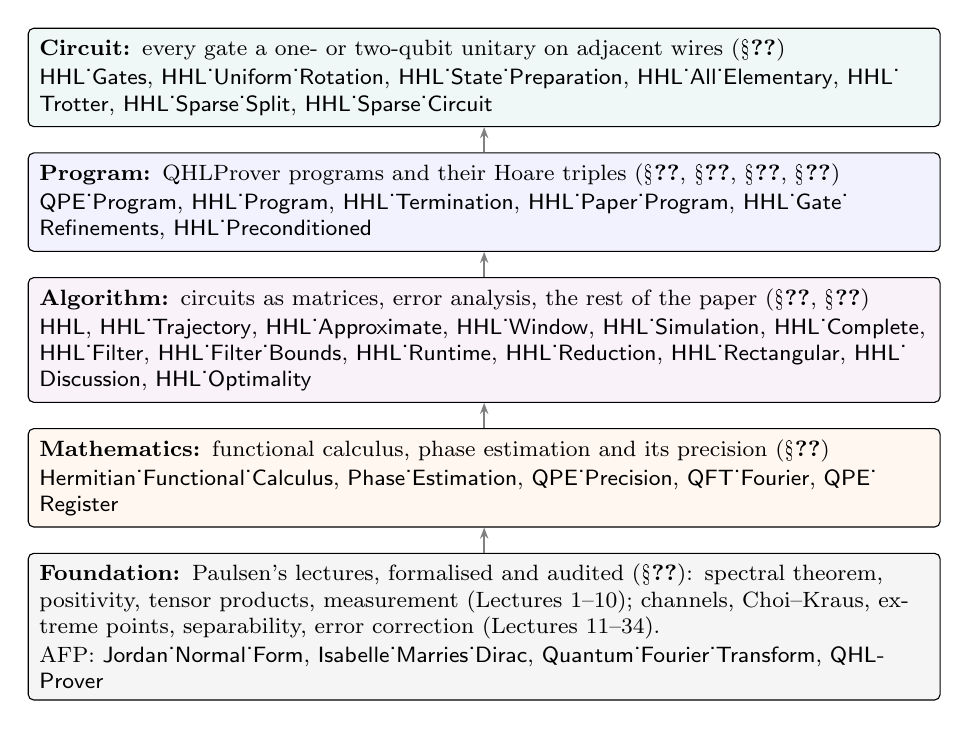
\begin{tikzpicture}[node distance=0.32cm,
  box/.style={draw, rounded corners=2pt, align=left, text width=11.3cm, inner sep=4pt, font=\footnotesize},
  arr/.style={-{Stealth[length=4pt]}, thick, gray}]
\node[box, fill=teal!6] (L4) {\textbf{Circuit:} every gate a one- or two-qubit unitary on adjacent wires
  (\S\ref{sec:gates})\\[1pt]
  \isa{HHL\_Gates}, \isa{HHL\_Uniform\_Rotation}, \isa{HHL\_State\_Preparation}, \isa{HHL\_All\_Elementary},
  \isa{HHL\_Trotter}, \isa{HHL\_Sparse\_Split}, \isa{HHL\_Sparse\_Circuit}};
\node[box, fill=blue!5, below=of L4] (L3) {\textbf{Program:} QHLProver programs and their Hoare triples
  (\S\ref{sec:qhl}, \S\ref{sec:qpe-program}, \S\ref{sec:exact}, \S\ref{sec:approx})\\[1pt]
  \isa{QPE\_Program}, \isa{HHL\_Program}, \isa{HHL\_Termination}, \isa{HHL\_Paper\_Program},
  \isa{HHL\_Gate\_Refinements}, \isa{HHL\_Preconditioned}};
\node[box, fill=violet!5, below=of L3] (L2) {\textbf{Algorithm:} circuits as matrices, error analysis,
  the rest of the paper (\S\ref{sec:exact}, \S\ref{sec:approx})\\[1pt]
  \isa{HHL}, \isa{HHL\_Trajectory}, \isa{HHL\_Approximate}, \isa{HHL\_Window}, \isa{HHL\_Simulation},
  \isa{HHL\_Complete}, \isa{HHL\_Filter}, \isa{HHL\_Filter\_Bounds}, \isa{HHL\_Runtime},
  \isa{HHL\_Reduction}, \isa{HHL\_Rectangular}, \isa{HHL\_Discussion}, \isa{HHL\_Optimality}};
\node[box, fill=orange!6, below=of L2] (L1) {\textbf{Mathematics:} functional calculus, phase estimation
  and its precision (\S\ref{sec:math})\\[1pt]
  \isa{Hermitian\_Functional\_Calculus}, \isa{Phase\_Estimation}, \isa{QPE\_Precision}, \isa{QFT\_Fourier},
  \isa{QPE\_Register}};
\node[box, fill=gray!8, below=of L1] (L0) {\textbf{Foundation:} Paulsen's lectures, formalised and audited
  (\S\ref{sec:paulsen}): spectral theorem, positivity, tensor products, measurement (Lectures 1--10);
  channels, Choi--Kraus, extreme points, separability, error correction (Lectures 11--34).\\[1pt]
  AFP: \isa{Jordan\_Normal\_Form}, \isa{Isabelle\_Marries\_Dirac}, \isa{Quantum\_Fourier\_Transform},
  \isa{QHLProver}};
\foreach \a/\b in {L0/L1, L1/L2, L2/L3, L3/L4} \draw[arr] (\a.north) -- (\b.south);
\end{tikzpicture}
\caption{The four levels of the HHL development and the theories at each level. Part VI of the
development has 31 theories; the foundation has 50.}\label{fig:layers}
\end{figure}

All results are checked by Isabelle2025-2 with \texttt{quick\_and\_dirty = false}, so no
\texttt{sorry} survives, and an audit with \isa{Thm\_Deps.all\_oracles} over all theorems of the
development finds no oracles. The sources, the generated documents and the audits are in the project
repository.\footnote{\url{https://github.com/brydustin/Quantum_Computing}} Each listing below links to
its source line (\isalogo).

The rest of the paper is organised as follows. Section~\ref{sec:qhl} recalls quantum Hoare logic and
explains how HHL's specifications read as triples. Section~\ref{sec:math} covers the functional
calculus and phase estimation, including its precision and its verification as a program.
Section~\ref{sec:exact} verifies exact HHL as a program, and Section~\ref{sec:approx} verifies inexact
HHL, in the regime of the paper's error analysis. Section~\ref{sec:gates}
compiles the programs to elementary gates, and Section~\ref{sec:errata} collects the errata.
Section~\ref{sec:paulsen} describes the foundation. Sections~\ref{sec:related}
and~\ref{sec:discussion} discuss related work, the trusted base and the limitations.
\section{Quantum Hoare Logic in Isabelle}\label{sec:qhl}

\subsection{States, Gates and Programs}

We use the concrete representation of the Jordan-Normal-Form library~\cite{thiemann2015jnf}, shared
by \IMD~\cite{bordg2021imd,bordg2020afp}, the quantum Fourier transform entry~\cite{manrique2025qft}
and QHLProver~\cite{liu2019qhl,liu2019afp}. A state is a vector \isa{v :: complex vec} with a
dimension hypothesis \isa{dim\_vec v = n}, an operator is a matrix with a carrier hypothesis
\isa{A $\in$ carrier\_mat n n}, $\otimes$ is the Kronecker product (\isa{tensor\_vec} for vectors),
$\ket j$ is the unit vector \isa{unit\_vec n j}, $\braket vw$ is antilinear in~$v$, and $A^\dagger$ is
the conjugate transpose. Dimensions are hypotheses rather than types, which is how the lecture notes
and the physics literature treat them, and which lets the libraries share their definitions. The
registers of HHL are ordered clock $\otimes$ system $\otimes$ ancilla, of dimensions $N=2^k$, $n$
and~$2$.

QHLProver formalises Ying's quantum while-language~\cite{ying2011,ying2016book}:
\[
S \;::=\; \mathbf{skip} \;\mid\; U \;\mid\; S_1;S_2 \;\mid\; \mathbf{measure}\ M\ [S_0,\dots,S_{m-1}]
\;\mid\; \mathbf{while}\ M\ \mathbf{do}\ S .
\]
A measurement is a family $M_0,\dots,M_{m-1}$ with $\sum_kM_k^\dagger M_k=I$, and a loop is controlled
by a two-outcome measurement. Programs act on partial density operators ($\rho\ge0$,
$\Tr\rho\le1$):
\begin{gather*}
\sem{U}\rho=U\rho U^\dagger,\qquad \sem{S_1;S_2}=\sem{S_2}\circ\sem{S_1},\\
\sem{\mathbf{measure}\ M\ \bar S}\rho=\textstyle\sum_k\sem{S_k}(M_k\rho M_k^\dagger),\\
\sem{\mathbf{while}\ M\ \mathbf{do}\ S}\rho=\textstyle\sum_{m\ge0}M_0\,\bigl((\sem S\circ\mathcal
M_1)^m\rho\bigr)\,M_0^\dagger,\quad\text{where } \mathcal M_1(\rho)=M_1\rho M_1^\dagger .
\end{gather*}
The loop runs $S$ on outcome~$1$ and exits on outcome~$0$, and the $m$-th summand is the part of the
input that exits after $m$ rounds. The meaning of a program is a completely positive,
trace-non-increasing map, and the trace lost by a loop is the probability that it does not terminate.

\subsection{Predicates and Triples}

A quantum predicate is an operator $0\le P\le I$. For a state $\rho$, $\Tr(P\rho)$ is the expected
value of the observable $P$; for a projector it is the probability that measuring $\{P,I-P\}$ yields
$P$. A triple compares these probabilities before and after the program (Listing~\ref{lst:triples}):
$\hoaret PSQ$ holds if $\Tr(P\rho)\le\Tr(Q\sem S\rho)$ for every input $\rho$, and partial correctness
adds the probability $\Tr\rho-\Tr\sem S\rho$ of not terminating to the right-hand side. These are
D'Hondt and Panangaden's predicates~\cite{dhondt2006} with Ying's notion of
correctness~\cite{ying2011}.

\noindent\begin{minipage}{\linewidth}
\begin{lstlisting}[caption={Quantum predicates and triples in QHLProver (inside the locale
\isa{state\_sig}, where \isa{d} is the dimension of the state space; syntax annotations
omitted)},label={lst:triples}]
definition is_quantum_predicate :: "complex mat ~$\Rightarrow$~ bool" where
  "is_quantum_predicate P ~$\longleftrightarrow$~ P ~$\in$~ carrier_mat d d ~$\wedge$~ positive P ~$\wedge$~ P ~$\le_{L}$~
      1~$_{m}$~ d"
definition hoare_total_correct :: "complex mat ~$\Rightarrow$~ com ~$\Rightarrow$~ complex mat
    ~$\Rightarrow$~ bool" where
  "~$\models_{t}$~ {P} S {Q} ~$\longleftrightarrow$~ (~$\forall\rho\in$~density_states. trace (P * ~$\rho$~) ~$\le$~ trace (Q *
      denote S ~$\rho$~))"
definition hoare_partial_correct :: "complex mat ~$\Rightarrow$~ com ~$\Rightarrow$~ complex
    mat ~$\Rightarrow$~ bool" where
  "~$\models_{p}$~ {P} S {Q} ~$\longleftrightarrow$~ (~$\forall\rho\in$~density_states.
      trace (P * ~$\rho$~) ~$\le$~ trace (Q * denote S ~$\rho$~) + (trace ~$\rho$~ - trace
          (denote S ~$\rho$~)))"
\end{lstlisting}
\end{minipage}

QHLProver also defines a proof system $\vdash_p$ for partial correctness and proves it sound and
complete~\cite{liu2019qhl}:
\begin{gather*}
\frac{}{\{U^\dagger PU\}\;U\;\{P\}}\quad\
\frac{\{P\}\,S_1\,\{Q\}\quad\{Q\}\,S_2\,\{R\}}{\{P\}\;S_1;S_2\;\{R\}}\quad\
\frac{P\le P'\quad\{P'\}\,S\,\{Q'\}\quad Q'\le Q}{\{P\}\;S\;\{Q\}}\\[0.5em]
\frac{\{P_k\}\,S_k\,\{Q\}\ \ (k<m)}{\{\sum_kM_k^\dagger P_kM_k\}\;\mathbf{measure}\ M\ \bar S\;\{Q\}}\qquad
\frac{\{Q\}\;S\;\{R\}}{\{R\}\;\mathbf{while}\ M\ \mathbf{do}\ S\;\{P\}}
\end{gather*}
where $R=M_0^\dagger PM_0+M_1^\dagger QM_1$ in the loop rule,
together with the rule for \textbf{skip}. The rules compute weakest preconditions backwards through
a program. For loop-free programs, partial and total correctness coincide because such programs
preserve the trace.

\subsection{HHL's Specification as Triples}

Every statement about HHL in this paper is a triple of one of four shapes
(Table~\ref{tab:readings}). Let $P_0$ and $P_1$ be the projectors onto ancilla value $0$ and~$1$
(\isa{anc\_proj}), and let $\ket t$ be a unit vector with $P_1\ket t=\ket t$, typically
$\ket t=\ket0\otimes A^{-1}b/\norm{A^{-1}b}\otimes\ket1$. Since $\Tr\rho=1$ for a state, a precondition
$q\cdot I$ asserts the number $q$ for every input. The second reading needs a short argument. Let
$\sigma=\sem S\rho$ for a state $\rho$. Then $\Tr\sigma\le1$, and $\Tr((P_0+\ketbra tt)\sigma)\ge1$
forces $\Tr((P_1-\ketbra tt)\sigma)\le0$. Since $P_1-\ketbra tt\ge0$, this gives
$P_1\sigma P_1=\bra t\sigma\ket t\,\ketbra tt$: whenever the ancilla reads~$1$, the state is
exactly~$\ket t$.

\begin{table}[t]
\caption{The four shapes of triple used for HHL, for a state $\rho$ with $\Tr\rho=1$.}\label{tab:readings}
\centering\small
\begin{tabular}{@{}l>{\raggedright\arraybackslash}p{6.9cm}@{}}
\toprule
Triple & Reading\\
\midrule
$\hoaret{p\cdot I}{S}{P_1}$ & $S$ terminates with the ancilla in $\ket1$ with probability $\ge p$\\
$\hoaret{I}{S}{P_0+\ketbra tt}$ & whenever the ancilla reads $1$ at the end, the state is exactly $\ket t$\\
$\hoaret{I}{S}{\ketbra tt}$ & $S$ terminates with probability one, in the state $\ket t$\\
$\hoaret{q\cdot I}{S}{\ketbra tt}$ & the output has fidelity at least $q$ with $\ket t$\\
\bottomrule
\end{tabular}
\end{table}

\subsection{What We Add to the Logic}

\paragraph{Initialisation.} QHLProver has no statement that prepares a fixed state. We build one from
a measurement in the computational basis followed by a permutation that moves the outcome~$k$
to~$0$. Its rule says that after \isa{init\_com} the probability of $Q$ is $\bra0Q\ket0$, whatever the
input.\isalink{Algorithms/HHL_Program.thy}{142}
\noindent\begin{minipage}{\linewidth}
\begin{lstlisting}[caption={Initialisation: a measurement and $K$ swaps, and its proof rule},label={lst:init}]
definition init_com :: "nat ~$\Rightarrow$~ com" where
  "init_com K = Measure K (proj_basis K) (map (~$\lambda$~k. Utrans (swap0 K
      k)) [0..<K])"
theorem hoare_init:
  assumes Q: "is_quantum_predicate Q" and d0: "0 < d"
  shows "~$\vdash_{p}$~ {Q ~\$\$~ (0, 0) ~$\cdot_{m}$~ 1~$_{m}$~ d} init_com d {Q}"
\end{lstlisting}
\end{minipage}

\paragraph{Gate lists.} A circuit $U_1,\dots,U_m$ becomes the program
$\isa{utrans\_seq}\,[U_1,\dots,U_m]=U_1;\dots;U_m$. All theorems about HHL programs are proved for
every list of unitaries whose product (\isa{circuit\_mat}) equals that of the eight gates of
Fig.~\ref{fig:hhl}. A refinement that replaces gates by circuits with the same product therefore
inherits every triple, which is how Section~\ref{sec:gates} reaches elementary gates.

\paragraph{Total correctness of loops.} The proof system covers partial correctness only. For loops
whose body re-initialises the state, we derive total correctness from the semantics
(Section~\ref{sec:rus}).

\paragraph{Fidelity triples.} For a program that initialises, runs a circuit and measures, the
probability of $\ketbra tt$ is the overlap $|\braket t\psi|^2$ with the circuit's output~$\psi$.
Section~\ref{sec:approx-programs} uses this to turn the error bounds of the algorithm into triples.
\section{Functional Calculus and Phase Estimation}\label{sec:math}

\subsection{A Functional Calculus for Hermitian Matrices}

HHL applies three functions to $A$: the evolution $e^{iAt}$, the inverse $A^{-1}$, and
$x\mapsto\sqrt{1-C^2/x^2}$, which appears in the output. We define $g(A)$ for Hermitian $A$ and any
$g:\R\to\C$ as the matrix that acts on every eigenvector by the value of $g$ at its eigenvalue
(Listing~\ref{lst:matfun}).

\begin{theorem}[functional calculus]\label{thm:matfun}
Let $A\in\C^{n\times n}$ be Hermitian. There is exactly one matrix $g(A)$ with $g(A)v=g(\lambda)v$ for
every eigenvector $v$ of $A$ with eigenvalue~$\lambda$, and $g(A)=U\operatorname{diag}(g(d_1),\dots,g(d_n))
U^\dagger$ for every spectral decomposition $U^\dagger AU=\operatorname{diag}(d_1,\dots,d_n)$.
\end{theorem}

Existence comes from the spectral theorem of Paulsen's Lecture~4
(\isa{hermitian\_spectral\_decomp}), and uniqueness from the fact that the eigenvectors span.
Multiplicativity $g(A)h(A)=(gh)(A)$, $g(A)^\dagger=\bar g(A)$, unitarity when $|g|=1$ on the spectrum,
and positivity when $g\ge0$ on it are all checked on eigenvectors. The instances are
$\isa{evolution}\ A\ t=e^{itA}$, with its group law, and $\isa{herm\_inv}\ A=A^{-1}$. Since $1/0=0$ in
HOL, \isa{herm\_inv} is the pseudo-inverse when $0$ is an eigenvalue (Section~\ref{sec:exact-other}).
The device behind the whole development is the following lemma: two matrices that agree on every
eigenvector of a Hermitian $A$ are equal (\isa{eigvec\_mat\_eqI}). It lets every statement about all
right-hand sides~$b$ be proved for an eigenvector, without sums over an eigenbasis.\isalink{Algorithms/Hermitian_Functional_Calculus.thy}{108}

\noindent\begin{minipage}{\linewidth}
\begin{lstlisting}[caption={The functional calculus},label={lst:matfun}]
definition fun_on_eigen :: "complex mat ~$\Rightarrow$~ (real ~$\Rightarrow$~ complex) ~$\Rightarrow$~
    complex mat ~$\Rightarrow$~ bool" where
  "fun_on_eigen A g B ~$\longleftrightarrow$~ (~$\forall$~v l. dim_vec v = dim_row A ~$\longrightarrow$~
     A *~$_{v}$~ v = complex_of_real l ~$\cdot_{v}$~ v ~$\longrightarrow$~ B *~$_{v}$~ v = g l ~$\cdot_{v}$~ v)"
definition mat_fun :: "(real ~$\Rightarrow$~ complex) ~$\Rightarrow$~ complex mat ~$\Rightarrow$~ complex
    mat" where
  "mat_fun g A = (SOME B. B ~$\in$~ carrier_mat (dim_row A) (dim_row A)
      ~$\wedge$~ fun_on_eigen A g B)"
theorem mat_fun_eigen:
  assumes A: "A ~$\in$~ carrier_mat n n" "hermitian A"
      and v: "dim_vec v = n" and ev: "A *~$_{v}$~ v = complex_of_real l ~$\cdot_{v}$~
          v"
  shows "mat_fun g A *~$_{v}$~ v = g l ~$\cdot_{v}$~ v"
theorem mat_fun_decomp:
  assumes A: "A ~$\in$~ carrier_mat n n" "hermitian A" and sd:
      "spectral_decomp A U D"
  shows "mat_fun g A = U * diag_cmat (map g D) * (U~$^{\dagger}$~)"
\end{lstlisting}
\end{minipage}

\subsection{Phase Estimation}

Let $F_N$ be the Fourier matrix, $(F_N)_{jk}=\omega^{jk}/\sqrt N$ with $\omega=e^{2\pi i/N}$, and let
$\Lambda(U)=\sum_c\ketbra cc\otimes U^c$ be the controlled powers of~$U$ (\isa{ctrl\_pow}). Phase
estimation is $(F_N^\dagger\otimes I)\Lambda(U)$ applied to the uniform clock state
$u=N^{-1/2}\sum_c\ket c$ (Fig.~\ref{fig:hhl}, gates~2--4).

\begin{theorem}[phase estimation]\label{thm:qpe}
If $Uv=e^{2\pi i\varphi}v$, then $(F_N^\dagger\otimes I)\Lambda(U)(u\otimes v)=(\sum_j\alpha_j\ket
j)\otimes v$ with $\alpha_j=\frac1N\sum_{k<N}e^{2\pi ik(\varphi-j/N)}$. If $\varphi=j_0/N$, then
$\alpha=\ket{j_0}$. If $|\varphi-j/N|\le1/(2N)$, then $|\alpha_j|^2\ge4/\pi^2$.
\end{theorem}

The first part is phase kickback: $\Lambda(U)(\ket c\otimes v)=e^{2\pi ic\varphi}\ket c\otimes v$. The
bound follows from the geometric sum, $|e^{ix}-1|=2|\sin(x/2)|$ and Jordan's inequality
$\sin x\ge2x/\pi$ on $[0,\pi/2]$. Two bridges connect the theorem to circuits. The quantum Fourier
transform circuit of the AFP~\cite{manrique2025qft} is the Fourier matrix (\isa{ordered\_QFT\_fourier},
by induction over its Kronecker structure), and $k$ Hadamard gates prepare the uniform state from
$\ket{0\cdots0}$ (\isa{hadamard\_layer\_zero}, from \IMD).\isalink{Algorithms/Phase_Estimation.thy}{291}

\noindent\begin{minipage}{\linewidth}
\begin{lstlisting}[caption={Phase estimation, the $4/\pi^2$ bound, and the bridges to circuits},label={lst:qpe}]
theorem phase_estimation:
  assumes U: "U ~$\in$~ carrier_mat m m" and u: "dim_vec u = m"
      and ev: "U *~$_{v}$~ u = cis (2 * pi * ~$\varphi$~) ~$\cdot_{v}$~ u"
  shows "(((fourier N)~$^{\dagger}$~) ~$\otimes$~ 1~$_{m}$~ m) *~$_{v}$~ (ctrl_pow N m U *~$_{v}$~ tensor_vec
      (uniform_state N) u) =
         tensor_vec (Matrix.vec N (pe_amp N ~$\varphi$~)) u"
theorem phase_estimation_bound:
  assumes N: "0 < N" and close: "~$|\varphi$~ - real j / real N~$|$~ ~$\le$~ 1 / (2 *
      real N)"
  shows "4 / pi~$^{2}$~ ~$\le$~ (cmod (pe_amp N ~$\varphi$~ j))~$^{2}$~"
theorem ordered_QFT_fourier: "ordered_QFT n = fourier (2 ^ n)"
theorem hadamard_layer_zero:
  assumes n: "1 ~$\le$~ n"
  shows "(Hadamard ~$\otimes^{n}$~) *~$_{v}$~ unit_vec (2 ^ n) 0 = uniform_state (2 ^
      n)"
\end{lstlisting}
\end{minipage}
\subsection{The Precision of Phase Estimation}\label{sec:qpe-precision}

Theorem~\ref{thm:qpe} bounds the probability of the best outcome from below. Choosing the size of the
clock needs the converse: distant outcomes must be unlikely. We measure the error of outcome~$j$ on the
circle $\R/\mathbb{Z}$, as the distance $d_j$ from $\varphi-j/N$ to the nearest integer (\isa{circ\_dist}), so
that phases close to $0$ and to $1$ count as close.

\begin{theorem}[precision of phase estimation]\label{thm:qpe-tail}
Let $N\ge1$ and $e>1$. For every phase~$\varphi$, the outcomes with $Nd_j>e$ have total probability
\[
\textstyle\sum_{Nd_j>e}|\alpha_j|^2\;\le\;\frac1{2(e-1)}.
\]
With $k=n+\lceil\log_2(2+1/(2\varepsilon))\rceil$ clock qubits, the outcome therefore satisfies
$d_j\le2^{-n}$ with probability at least $1-\varepsilon$.
\end{theorem}

This is Eq.~(5.34) of Nielsen and Chuang and the choice of the clock size after
it~\cite[Sect.~5.2.1]{nielsenchuang}; Fig.~\ref{fig:qpe} shows an instance. The proof has two steps. The
geometric sum gives $|\alpha_j|\le1/(2Nd_j)$ (\isa{pe\_amp\_circ\_tail}). The signed errors $y_j$, which are
$N(\varphi-j/N)$ reduced into $[-\frac N2,\frac N2]$, differ by nonzero integers for distinct outcomes.
So $j\mapsto\lceil y_j-e\rceil$ is injective on the outcomes with $y_j>e$, and
$y_j>e+\lceil y_j-e\rceil-1$. Telescoping gives
$\sum_{y_j>e}y_j^{-2}\le\sum_{m\ge1}(e+m-1)^{-2}\le1/(e-1)$ (\isa{sum\_inv\_sq\_spaced}). The same holds
below $-e$, and the two halves give $\frac14\cdot\frac2{e-1}$. For the second part, $\sum_j|\alpha_j|^2=1$
and $e=2^{k-n}\ge2+1/(2\varepsilon)$.\isalink{Algorithms/QPE_Precision.thy}{187}

\noindent\begin{minipage}{\linewidth}
\begin{lstlisting}[caption={Theorem~\ref{thm:qpe-tail}},label={lst:qpetail}]
definition wrap :: "real ~$\Rightarrow$~ real" where
  "wrap x = x - of_int (round x)"
definition circ_dist :: "real ~$\Rightarrow$~ real ~$\Rightarrow$~ real" where
  "circ_dist x y = ~$|$~wrap (x - y)~$|$~"
theorem pe_tail_bound:
  assumes N: "0 < N" and e: "1 < e"
  shows "(~$\sum$~j | j < N ~$\wedge$~ e < real N * circ_dist ~$\varphi$~ (real j /
      real N). (cmod (pe_amp N ~$\varphi$~ j))~$^{2}$~) ~$\le$~ 1 / (2 * (e - 1))"
theorem pe_precision:
  assumes eps: "0 < ~$\varepsilon$~"
      and t: "t = n + nat ~$\lceil$~log 2 (2 + 1 / (2 * ~$\varepsilon$~))~$\rceil$~"
  shows "1 - ~$\varepsilon$~ ~$\le$~ (~$\sum$~j | j < 2 ^ t ~$\wedge$~ circ_dist ~$\varphi$~ (real j /
      2 ^ t) ~$\le$~ 1 / 2 ^ n. (cmod (pe_amp (2 ^ t) ~$\varphi$~ j))~$^{2}$~)"
\end{lstlisting}
\end{minipage}

\begin{figure}[t]
\centering
\scalebox{0.85}{%
\begin{quantikz}[row sep={0.8cm,between origins}, column sep=0.3cm]
\lstick{clock $\ket{0}^{\otimes k}$} & \qwbundle{k} & & \gate{H^{\otimes k}} & \ctrl{1} &
  \gate{F^\dagger} & \meter{} \rstick{$j$}\\
\lstick{system $\ket{0}^{\otimes s}$} & \qwbundle{s} & \gate{U_u} & & \gate{U^{c}} & & \rstick{$u$}
\end{quantikz}}
\\[0.4em]
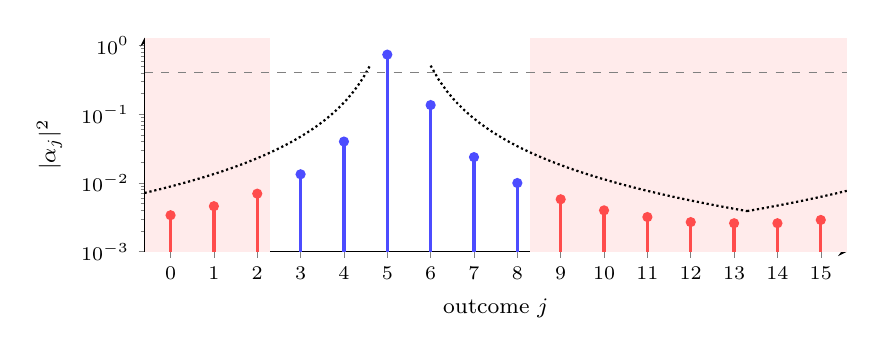
\begin{tikzpicture}
\begin{axis}[width=10.5cm, height=4.3cm, ymode=log, log origin y=infty, ymin=1e-3, ymax=1.3,
  xmin=-0.6, xmax=15.6,
  axis lines=left, xtick={0,...,15}, ytick={0.001,0.01,0.1,1},
  xlabel={outcome $j$}, ylabel={$|\alpha_j|^2$}, tick label style={font=\scriptsize},
  label style={font=\footnotesize}]
\fill[red!8] (axis cs:-0.6,0.001) rectangle (axis cs:2.3,1.3);
\fill[red!8] (axis cs:8.3,0.001) rectangle (axis cs:15.6,1.3);
\addplot[densely dotted, thick, domain=-0.6:4.6, samples=40] {1/(4*(5.3-x)^2)};
\addplot[densely dotted, thick, domain=6:13.3, samples=40] {1/(4*(x-5.3)^2)};
\addplot[densely dotted, thick, domain=13.3:15.6, samples=10] {1/(4*(21.3-x)^2)};
\addplot[dashed, gray, domain=-0.6:15.6, samples=2] {4/pi^2};
\addplot[ycomb, very thick, blue!70, mark=*, mark size=1.2pt] coordinates
  {(3,0.0134) (4,0.0401) (5,0.7377) (6,0.1362) (7,0.0238) (8,0.0100)};
\addplot[ycomb, very thick, red!70, mark=*, mark size=1.2pt] coordinates
  {(0,0.0034) (1,0.0046) (2,0.0070) (9,0.0058) (10,0.0040) (11,0.0032) (12,0.0027) (13,0.0026)
   (14,0.0026) (15,0.0029)};
\end{axis}
\end{tikzpicture}
\caption{Phase estimation as a program (top), and its outcome distribution for $N=16$ and
$N\varphi=5.3$ (bottom, logarithmic scale). The nearest value $j=5$ has probability $0.74\ge4/\pi^2$
(dashed line). The dotted curve is the tail bound $|\alpha_j|^2\le1/(4N^2d_j^2)$. The outcomes more than
$e=3$ from $N\varphi$ (shaded) have total probability $0.039$, below the bound $1/(2(e-1))=\frac14$ of
Theorem~\ref{thm:qpe-tail}.}\label{fig:qpe}
\end{figure}

\subsection{Phase Estimation as a Program}\label{sec:qpe-program}

Before HHL, phase estimation itself shows how probabilistic guarantees become triples. The program
\isa{qpe\_program} initialises the state, prepares an eigenvector $u=U_u\ket0$ of~$U$ in the system
register, and applies the gates of Theorem~\ref{thm:qpe} (Fig.~\ref{fig:qpe}, top). For a set $J$ of
clock values, the predicate $\Pi_J=\sum_{j\in J}\ketbra jj\otimes I$ (\isa{clock\_proj}) holds when the
clock reads a value in~$J$.

\begin{theorem}[phase estimation as a program]\label{thm:qpe-prog}
Let $U$ and $U_u$ be unitary, $u=U_u\ket0$, $Uu=e^{2\pi i\varphi}u$ and $N=2^k$. For every set $J$ of
clock values,
\[
\hoaret{\textstyle\bigl(\sum_{j\in J}|\alpha_j|^2\bigr)\,I}{\mathit{QPE}}{\Pi_J},
\]
and on every input $\rho$ the probability of $\Pi_J$ is exactly $\sum_{j\in J}|\alpha_j|^2\Tr\rho$, so no
larger multiple of $I$ is a precondition. In particular:
\begin{enumerate}
\item if $\varphi=j_0/N$ with $j_0<N$, then $\hoaret{I}{\mathit{QPE}}{\Pi_{\{j_0\}}}$;
\item for every $\varphi$, $\hoaret{(4/\pi^2)\,I}{\mathit{QPE}}{\Pi_{\{j^*\}}}$, where
$j^*=\mathrm{round}(N\varphi)\bmod N$;
\item if $k=n+\lceil\log_2(2+1/(2\varepsilon))\rceil$, then
$\hoaret{(1-\varepsilon)\,I}{\mathit{QPE}}{\Pi_{\{j\,:\,d_j\le2^{-n}\}}}$.
\end{enumerate}
The first triple also holds for the program whose gates are $k$ Hadamard gates, one controlled
$U^{2^j}$ per clock qubit and the inverted Fourier circuit of the AFP.
\end{theorem}

The program initialises and then runs a unitary circuit, so its semantics maps every $\rho$ to
$\Tr\rho\,\ketbra\psi\psi$, where $\psi=(\sum_j\alpha_j\ket j)\otimes u$ by Theorem~\ref{thm:qpe} and
\isa{hadamard\_layer\_zero} (\isa{qpe\_out}, \isa{qpe\_prob}). The rule for initialisation and the gate
rules of Section~\ref{sec:qhl} give the triple with the precondition $\bra\psi\Pi_J\ket\psi\,I$, and
$\bra\psi\Pi_J\ket\psi=\sum_{j\in J}|\alpha_j|^2$ because $u$ is a unit vector (\isa{clock\_proj\_value}).
Soundness gives the semantic triple, and the program has no loop, so partial and total correctness
agree. Items (1)--(3) weaken the precondition by Theorems~\ref{thm:qpe} and~\ref{thm:qpe-tail}; for~(2),
$j^*$ is within $\frac1{2N}$ of $\varphi$ on the circle, and the periodicity of $\alpha_j$ in $\varphi$
reduces this to Theorem~\ref{thm:qpe} (\isa{pe\_round\_dist}, \isa{pe\_amp\_near}). In the gate-level
program the Hadamard gates multiply to $H^{\otimes k}$ (\isa{had\_gates}), the controlled powers to
$\Lambda(U)$ (\isa{ctrl\_pow\_qubits}) and the inverted gate list to $F_N^\dagger$
(\isa{qft\_inv\_circuit}). The triples of an initialised circuit depend only on the product of its
gates (\isa{init\_circuit\_transfer}, \isa{qpe\_elem\_total}).\isalink{Algorithms/QPE_Program.thy}{177}

\begin{lstlisting}[float=tp, caption={Theorem~\ref{thm:qpe-prog} (\isa{Js} is the set $J$)},label={lst:qpeprog}]
definition qpe_program :: "nat ~$\Rightarrow$~ complex mat ~$\Rightarrow$~ complex mat ~$\Rightarrow$~
    com" where
  "qpe_program k U Uu = init_com (2 ^ k * dim_row U) ;; utrans_seq
      (qpe_gates k U Uu)"
context
  fixes U Uu :: "complex mat" and u :: "complex vec" and m k :: nat
      and ~$\varphi$~ :: real
  assumes U: "U ~$\in$~ carrier_mat m m" "unitary U" and m0: "0 < m"
      and k: "1 ~$\le$~ k"
    and Uu: "Uu ~$\in$~ carrier_mat m m" "unitary Uu" "Uu *~$_{v}$~ unit_vec m 0
        = u"
    and ev: "U *~$_{v}$~ u = cis (2 * pi * ~$\varphi$~) ~$\cdot_{v}$~ u"
begin
theorem qpe_total:
  "state_sig.hoare_total_correct [2 ^ k, m]
     (complex_of_real (~$\sum$~j | j < 2 ^ k ~$\wedge$~ j ~$\in$~ Js. (cmod (pe_amp
         (2 ^ k) ~$\varphi$~ j))~$^{2}$~) ~$\cdot_{m}$~ 1~$_{m}$~ (2 ^ k * m))
     (qpe_program k U Uu) (clock_proj (2 ^ k) m Js)"
corollary qpe_nearest_total:
  "state_sig.hoare_total_correct [2 ^ k, m] (complex_of_real (4 /
      pi~$^{2}$~) ~$\cdot_{m}$~ 1~$_{m}$~ (2 ^ k * m))
     (qpe_program k U Uu) (clock_proj (2 ^ k) m {pe_round (2 ^ k)
         ~$\varphi$~})"
corollary qpe_precision_total:
  assumes eps: "0 < ~$\varepsilon$~"
      and t: "k = n + nat ~$\lceil$~log 2 (2 + 1 / (2 * ~$\varepsilon$~))~$\rceil$~"
  shows "state_sig.hoare_total_correct [2 ^ k, m] (complex_of_real (1
      - ~$\varepsilon$~) ~$\cdot_{m}$~ 1~$_{m}$~ (2 ^ k * m))
     (qpe_program k U Uu) (clock_proj (2 ^ k) m {j. circ_dist ~$\varphi$~
         (real j / 2 ^ k) ~$\le$~ 1 / 2 ^ n})"
\end{lstlisting}

\section{Exact HHL as a Verified Program}\label{sec:exact}

In this section every eigenvalue of $A$ is a grid value: $\lambda_k=2\pi k/(Nt_0)$ for $k<N/2$ and
$2\pi(k-N)/(Nt_0)$ otherwise (\isa{reg\_eig}), so that $e^{it_0\lambda_k}=\omega^k$ and phase
estimation is exact. This is the setting of the Coq proofs~\cite{zhou2023coqq,wu2024local};
Section~\ref{sec:approx} removes it. The HHL program extends the phase-estimation program of
Section~\ref{sec:qpe-program} by the controlled rotation, the uncomputation and a measurement of an
ancilla.

\subsection{The Circuit}

The circuit is $W^\dagger RW$, with phase estimation $W=(F_N^\dagger\otimes I)\Lambda(e^{iAt_0}\otimes I)$
and the controlled rotation $R=\sum_k\ketbra kk\otimes I\otimes R(C/\lambda_k)$. Here
$R(c)=\left(\begin{smallmatrix}\sqrt{1-c^2}&-c\\c&\sqrt{1-c^2}\end{smallmatrix}\right)$ is unitary for
$|c|\le1$.

\begin{theorem}[exact HHL]\label{thm:hhl}
Let $A\in\C^{n\times n}$ be Hermitian with every eigenvalue a nonzero grid value $\lambda_k$, $0<k<N$.
Then for every $b\in\C^n$ and every real $C$,
\[
W^\dagger RW\,(u\otimes b\otimes\ket0)=u\otimes\bigl(\sqrt{I-C^2A^{-2}}\,b\otimes\ket0+CA^{-1}b\otimes\ket1\bigr).
\]
Hence $x=A^{-1}b$ solves $Ax=b$, the ancilla reads $1$ with probability $C^2\norm x^2$, and if
$C\le|\lambda|\le\Lambda$ on the spectrum, this probability is at least $(C/\Lambda)^2\norm b^2$, which
is $1/\kappa^2$ for unit $b$ and $C=\lambda_{\min}$.\isalink{Algorithms/HHL.thy}{593}
\end{theorem}

\noindent\begin{minipage}{\linewidth}
\begin{lstlisting}[caption={Exact HHL as a matrix identity, for every right-hand side},label={lst:hhl}]
theorem hhl:
  assumes A: "A ~$\in$~ carrier_mat n n" "hermitian A" and t0: "0 < t0"
      and N: "0 < N"
      and spec: "~$\bigwedge$~l. l ~$\in$~ herm_spectrum A ~$\Longrightarrow$~ ~$\exists$~k. 0 < k ~$\wedge$~ k < N ~$\wedge$~ l =
          reg_eig t0 N k"
      and b: "dim_vec b = n"
  shows "hhl_circuit A t0 N C *~$_{v}$~ tensor_vec (uniform_state N)
      (tensor_vec b (unit_vec 2 0)) =
         tensor_vec (uniform_state N)
           (tensor_vec (mat_fun (~$\lambda$~x. complex_of_real (sqrt (1 - (C
               / x)~$^{2}$~))) A *~$_{v}$~ b) (unit_vec 2 0) +
            tensor_vec ((complex_of_real C ~$\cdot_{m}$~ herm_inv A) *~$_{v}$~ b)
                (unit_vec 2 1))"
\end{lstlisting}
\end{minipage}

The proof first takes $b$ to be an eigenvector with eigenvalue $\lambda_k$
(\isa{hhl\_eigen}). Phase estimation sends $u\otimes b$ to $\ket k\otimes b$ by
Theorem~\ref{thm:qpe}, the rotation acts on the single branch~$k$, and $W^\dagger$ undoes~$W$. Both
sides of the identity are linear in $b$ and of the form $Mb$ for matrices $M$ built with
\isa{lift\_mat}, so \isa{eigvec\_mat\_eqI} extends the identity to all~$b$. The success bound applies
the functional calculus to $g(x)=1/x^2-1/\Lambda^2$, which is non-negative on the spectrum, so $g(A)$ is
positive (\isa{hhl\_success\_bound}).

\subsection{The Program and its Trajectory}

As a program, HHL starts from $\ket{0}\ket{0}\ket{0}$. It prepares $\ket b=U_b\ket0$ and the uniform
clock with Hadamard gates, so the circuit has eight gates (\isa{hhl\_gates}, Fig.~\ref{fig:hhl}). The
table of Fig.~\ref{fig:hhl} is the theorem \isa{hhl\_steps}, which gives the state after each gate for
every~$b$. Phase estimation leaves $\sum_j\ket j\otimes\Pi_jb\otimes\ket0$, where $\Pi_j=g_j(A)$ for the
indicator $g_j$ of $\{\lambda_j\}$. With the unitary rule and the rule of consequence, each line
becomes a triple $\{\ketbra{\psi_i}{\psi_i}\}\,U_i\,\{\ketbra{\psi_{i+1}}{\psi_{i+1}}\}$
(\isa{hhl\_step\_triples}). The program initialises all registers, runs the gates and measures the
ancilla (Listing~\ref{lst:prog}).\isalink{Algorithms/HHL_Program.thy}{565}

\begin{lstlisting}[float=tp,caption={The programs for a gate list and a two-outcome measurement: one run, and repeat until the outcome is $1$. HHL measures the ancilla},label={lst:prog}]
definition prog_meas :: "nat ~$\Rightarrow$~ (nat ~$\Rightarrow$~ complex mat) ~$\Rightarrow$~ complex mat list
    ~$\Rightarrow$~ com" where
  "prog_meas K M Us = init_com K ;; utrans_seq Us ;; Measure 2 M
      [SKIP, SKIP]"
definition rus_meas :: "nat ~$\Rightarrow$~ (nat ~$\Rightarrow$~ complex mat) ~$\Rightarrow$~ complex mat list
    ~$\Rightarrow$~ com" where
  "rus_meas K M Us = init_com K ;; utrans_seq Us ;;
                     While (~$\lambda$~j. M (1 - j)) (init_com K
                         ;; utrans_seq Us)"
abbreviation hhl_prog :: "nat ~$\Rightarrow$~ complex mat list ~$\Rightarrow$~ com" where
  "hhl_prog K Us ~$\equiv$~ prog_meas K (anc_proj K) Us"
abbreviation hhl_rus_prog :: "nat ~$\Rightarrow$~ complex mat list ~$\Rightarrow$~ com" where
  "hhl_rus_prog K Us ~$\equiv$~ rus_meas K (anc_proj K) Us"
definition hhl_program :: "complex mat ~$\Rightarrow$~ complex mat ~$\Rightarrow$~ real ~$\Rightarrow$~ nat
    ~$\Rightarrow$~ real ~$\Rightarrow$~ com" where
  "hhl_program A Ub t0 k C = hhl_prog (2 ^ k * (dim_row A * 2))
      (hhl_gates A Ub t0 k C)"
\end{lstlisting}

\begin{theorem}[exact HHL, one run]\label{thm:prog}
Let $A$ be as in Theorem~\ref{thm:hhl} with $N=2^k$, let $U_b$ be a unitary with $U_b\ket0=b$, and let
$|C/\lambda_j|\le1$ for all $j<N$. Let $p=C^2\norm{A^{-1}b}^2$ and
$\ket t=\ket0\otimes A^{-1}b/\norm{A^{-1}b}\otimes\ket1$. Then
\[
\hoaret{p\cdot I}{\mathit{hhl\_program}}{P_1}\qquad\text{and}\qquad
\hoaret{I}{\mathit{hhl\_program}}{P_0+\ketbra tt}.
\]
\end{theorem}

By Table~\ref{tab:readings}, a single run succeeds with probability at least~$p$, and on success the
state is exactly~$\ket t$. The hypothesis on $C$ makes the rotation gate unitary, as the program
semantics requires. Listing~\ref{lst:progthm} shows the formal statement, including the context that
fixes the hypotheses.\isalink{Algorithms/HHL_Program.thy}{1192}

\noindent\begin{minipage}{\linewidth}
\begin{lstlisting}[caption={Theorem~\ref{thm:prog} (\isa{state\_sig.hoare\_total\_correct dims} is $\models_t$ on the registers \isa{dims})},label={lst:progthm}]
context
  fixes A Ub :: "complex mat" and b :: "complex vec" and n k ::
      nat and t0 C :: real
  assumes A: "A ~$\in$~ carrier_mat n n" "hermitian A" and n0: "0 < n"
      and k: "1 ~$\le$~ k" and t0: "0 < t0"
    and spec: "~$\bigwedge$~l. l ~$\in$~ herm_spectrum A ~$\Longrightarrow$~ ~$\exists$~j. 0 < j ~$\wedge$~ j < 2 ^ k ~$\wedge$~ l
        = reg_eig t0 (2 ^ k) j"
    and Ub: "Ub ~$\in$~ carrier_mat n n" "unitary Ub" "Ub *~$_{v}$~ unit_vec n
        0 = b"
    and Cb: "~$\bigwedge$~j. j < 2 ^ k ~$\Longrightarrow$~ ~$|$~C / reg_eig t0 (2 ^ k) j~$|$~ ~$\le$~ 1"
begin
theorem hhl_success_total:
  "state_sig.hoare_total_correct [2 ^ k, n, 2]
     (complex_of_real (C~$^{2}$~ * ~$\|$~herm_inv A *~$_{v}$~ b~$\|^{2}$~) ~$\cdot_{m}$~ 1~$_{m}$~ (2 ^ k * (n
         * 2)))
     (hhl_program A Ub t0 k C) (anc_proj (2 ^ k * (n * 2)) 1)"
theorem hhl_correct_total:
  "state_sig.hoare_total_correct [2 ^ k, n, 2] (1~$_{m}$~ (2 ^ k * (n *
      2))) (hhl_program A Ub t0 k C)
     (anc_proj (2 ^ k * (n * 2)) 0 + outer_prod (hhl_target A k b)
         (hhl_target A k b))"
\end{lstlisting}
\end{minipage}

The partial-correctness versions are derived with the proof rules (\isa{hhl\_success},
\isa{hhl\_correct}). The postcondition is pulled back through the measurement with the measurement
rule, through the gates with the unitary rule, which along the trajectory turns it into a predicate
whose value on $\ket{000}$ is $p$ (respectively~$1$), and through the initialisation with
\isa{hoare\_init}. Total correctness follows because programs without loops preserve the trace
(\isa{denote\_trace\_eq}). All of this is proved for any gate list with the circuit of the eight
gates (\isa{hhl\_prog\_success}, \isa{hhl\_prog\_correct}).

\subsection{Repeat Until Success}\label{sec:rus}

A failed run (ancilla~$0$) is discarded and the program is run again. This is the loop
\isa{hhl\_rus\_prog} of Listing~\ref{lst:prog}, which exits when the ancilla reads~$1$. Partial
correctness, $\hoarep{I}{\mathit{hhl\_rus}}{\ketbra tt}$ (\isa{hhl\_rus\_correct}), follows from the
loop rule. Its invariant is $P_0+\ketbra tt$, the postcondition of the second triple of
Theorem~\ref{thm:prog}. It says nothing about termination,
and QHLProver has no rule for total correctness of loops. We therefore work in the semantics.
Because the body begins with \isa{init\_com}, it maps every input $\rho$ to $(\Tr\rho)\,\sigma$ for the
fixed state $\sigma=\sem{\mathit{init};U_1;\dots;U_8}(\ketbra00)$. The $m$-th summand of the loop
semantics is then $(1-p)^m$ times the exit of one round, and the loop is a geometric series.

\begin{lemma}[loops with a resetting body]\label{lem:reset}
Let $M$ be a two-outcome measurement and $S$ a body with $\sem S\rho=(\Tr\rho)\,\sigma$ for every
partial density operator $\rho$, where $\Tr\sigma=1$, $\Tr(M_1\sigma M_1^\dagger)=1-p$ and $0<p\le1$.
Let $Q$ be a predicate and $v=\Tr(QM_0\sigma M_0^\dagger)$. Then
$\Tr\bigl(Q\,\sem{\mathbf{while}\ M\ \mathbf{do}\ S}(c\sigma)\bigr)\ge cv/p$ for $0\le c\le1$.\isalink{Algorithms/HHL_Termination.thy}{220}
\end{lemma}

\noindent\begin{minipage}{\linewidth}
\begin{lstlisting}[caption={Lemma~\ref{lem:reset}},label={lst:reset}]
lemma while_reset_total:
  assumes M: "measurement d 2 M" and Sc: "well_com Sc"
    and ~$\sigma$~: "~$\sigma$~ ~$\in$~ carrier_mat d d" "partial_density_operator ~$\sigma$~"
        "trace ~$\sigma$~ = 1"
    and reset: "~$\bigwedge\rho$~. ~$\rho$~ ~$\in$~ carrier_mat d d ~$\Longrightarrow$~ partial_density_operator
        ~$\rho$~ ~$\Longrightarrow$~ denote Sc ~$\rho$~ = trace ~$\rho$~ ~$\cdot_{m}$~ ~$\sigma$~"
    and p: "trace (M 1 * ~$\sigma$~ * adjoint (M 1)) = complex_of_real (1 -
        p)" "0 < p" "p ~$\le$~ 1"
    and Q: "is_quantum_predicate Q" and v: "trace (Q * (M 0 * ~$\sigma$~ *
        adjoint (M 0))) = complex_of_real v"
    and c: "0 ~$\le$~ c" "c ~$\le$~ 1"
  shows "complex_of_real (c * v / p) ~$\le$~ trace (Q * denote (While M
      Sc) (complex_of_real c ~$\cdot_{m}$~ ~$\sigma$~))"
\end{lstlisting}
\end{minipage}

For HHL, $M_0=P_1$ and the exit of one round is $p\,\ketbra tt$, so $Q=\ketbra tt$ gives $v=p$. The
probability of $\ket t$ at the end is then at least the trace of the input, which is total
correctness.

\begin{theorem}[exact HHL, repeat until success]\label{thm:rus}
Under the hypotheses of Theorem~\ref{thm:prog} and $C\neq0$:
\begin{enumerate}
\item $\hoaret{I}{\mathit{hhl\_rus}}{\ketbra tt}$, i.e.\ the loop terminates with probability one in~$\ket t$;
\item after exactly $m$ failed rounds the loop exits with probability $(1-p)^mp$, in the state $\ket t$,
and is still running with probability $(1-p)^m$;
\item the expected number of rounds is $\sum_m(m+1)p(1-p)^m=1/p$.\isalink{Algorithms/HHL_Termination.thy}{466}
\end{enumerate}
\end{theorem}

\noindent\begin{minipage}{\linewidth}
\begin{lstlisting}[caption={Theorem~\ref{thm:rus}(1) and~(3), in the context of Listing~\ref{lst:progthm}},label={lst:rus}]
theorem hhl_rus_total:
  assumes "C ~$\neq$~ 0"
  shows "state_sig.hoare_total_correct [2 ^ k, n, 2] (1~$_{m}$~ (2 ^ k *
      (n * 2))) (hhl_rus A Ub t0 k C)
     (outer_prod (hhl_target A k b) (hhl_target A k b))"
theorem hhl_rus_expected_rounds:
  assumes C0: "C ~$\neq$~ 0"
  defines "p ~$\equiv$~ C~$^{2}$~ * ~$\|$~herm_inv A *~$_{v}$~ b~$\|^{2}$~"
  shows "(~$\lambda$~m. real (Suc m) * (p * (1 - p) ^ m)) sums (1 / p)" and
      "(~$\lambda$~m. (1 - p) ^ m) sums (1 / p)"
\end{lstlisting}
\end{minipage}

Part~(2) is \isa{hhl\_rus\_prog\_rounds}, which computes the $m$-th iterate of the loop semantics
in closed form. With $C=\lambda_{\min}$ and unit $b$, the expected number of rounds is at most
$\kappa^2$; amplitude amplification reduces this to $O(\kappa)$ (Section~\ref{sec:approx}).

\subsection{Running the Circuit}\label{sec:run}

The semantics of programs is denotational and $g(A)$ is defined by choice, so \isa{hhl\_program}
cannot be evaluated as it stands. Its circuit can, once $A$ is concrete. Take
\[
A=\begin{pmatrix}2&1\\1&2\end{pmatrix},\qquad b=\ket0,\qquad k=3,\qquad t_0=\pi/4,\qquad C=1.
\]
Then $H^\dagger AH=\mathrm{diag}(3,1)$, so the eigenvalues sit on the clock values $3$ and $1$, and
$e^{iAt_0}=H\,\mathrm{diag}(\omega^3,\omega)\,H^\dagger$ with $\omega=e^{i\pi/4}$
(\isa{demo\_evolution}, by \isa{mat\_fun\_decomp}). Every amplitude lies in $\mathbb Q(i,\sqrt2)$.
With exact arithmetic in $\mathbb Q(\sqrt b)$ from the AFP~\cite{thiemann2014realimpl}, matrices as
arrays, and index formulas for the tensor products, Isabelle's \isa{value} command runs the eight
gates in a few seconds and prints the nine states. Three of them, as
$\ket{\text{clock}}\ket{\text{system}}\ket{\text{ancilla}}$:
\begin{align*}
\psi_4&=\tfrac12\ket1(\ket0-\ket1)\ket0+\tfrac12\ket3(\ket0+\ket1)\ket0,\\
\psi_5&=\tfrac12\ket1(\ket0-\ket1)\ket1+\ket3(\ket0+\ket1)\big(\tfrac{\sqrt2}3\ket0+\tfrac16\ket1\big),\\
\psi_8&=\ket0\Big(\tfrac{\sqrt2}3(\ket0+\ket1)\ket0+\big(\tfrac23\ket0-\tfrac13\ket1\big)\ket1\Big).
\end{align*}
After phase estimation the clock holds the eigenvalue of each component of $b$; the rotation sends
the $\lambda=1$ part to ancilla~$1$ entirely and the $\lambda=3$ part with amplitude $1/3$; after
uncomputation the ancilla-$1$ branch is $A^{-1}b=(\tfrac23,-\tfrac13)$, read with probability
$\tfrac59$.

The printed states are theorems. The gate list is the instance of \isa{hhl\_gates}, and its $i$-th
prefix produces \isa{hhl\_states}$\,!\,i$ (Listing~\ref{lst:demo}), so the run is an instance of
\isa{hhl\_steps}; \isa{demo\_output} states $\psi_8$. Theorem~\ref{thm:prog} specialises to this
program with $p=\tfrac59$ and $\ket t=\ket0\otimes(2,-1)/\sqrt5\otimes\ket1$ (\isa{demo\_correct},
\isa{demo\_success}). The code equations are proved, so \isa{value} evaluates the verified
definitions; only the evaluation itself is trusted to the code generator, and no theorem depends on
it. The example is a separate session, as \cite{thiemann2014realimpl} replaces the code setup of the
reals.\isalink{Demo/HHL_Demo.thy}{169}

\begin{lstlisting}[float=tp,caption={The example run: the gate list is the instance, each prefix gives the trajectory's state, and \isa{value} prints the states},label={lst:demo}]
theorem demo_gates_eq:
  "hhl_gates demo_A (1~$_{m}$~ 2) (pi / 4) 3 1 = demo_gates"
theorem demo_trajectory:
  "i ~$\le$~ 8 ~$\Longrightarrow$~ run_gates (unit_vec 32 0) (take i demo_gates)
                 = hhl_states demo_A (unit_vec 2 0) (pi / 4) 3 1 ! i"
value [code] "demo_trace"
\end{lstlisting}

\subsection{Other Systems}\label{sec:exact-other}

For an invertible non-Hermitian $A$, the program runs on the Hermitian dilation
$\tilde A=\left(\begin{smallmatrix}0&A\\A^\dagger&0\end{smallmatrix}\right)$, and $\tilde A^{-1}$ maps
$b\oplus0$ to $0\oplus x$ (\isa{herm\_embed\_inverse}). A preconditioned system $BAx=Bb$ is run in the
same way. On success the system register holds $0\oplus x/\norm x$ for the solution of the original
$Ax=b$, and the success probability is at least $(C/s)^2$ when $\norm{BAv}\le s\norm v$
(\isa{hhl\_elem\_precond\_correct}, \isa{hhl\_elem\_precond\_bound}). For a rectangular
$A\in\C^{M\times N}$, the pseudo-inverse of the dilation maps $b\oplus0$ to $0\oplus x$ with
$A^\dagger Ax=A^\dagger b$ and $x$ in the range of $A^\dagger$. So $x$ is the minimum-norm solution
when $Ax=b$ is solvable, and a least-squares solution otherwise (\isa{pinv\_solution},
\isa{normal\_eq\_least\_squares}). The proof uses $Jg(H)J=g(-H)$ for the parity~$J$, and it is here
that $1/0=0$, which makes \isa{herm\_inv} the pseudo-inverse, pays off.
\section{Inexact HHL: the Paper's Error Analysis}\label{sec:approx}

Section~\ref{sec:exact} assumed that every eigenvalue lies on the phase-estimation grid. In general the
eigenvalues of $A$ lie anywhere in a spectral window, $e^{iAt_0}$ is available only approximately, and
the success probability must be amplified. This section verifies this inexact case. It follows the
paper's analysis~\cite[App.~A]{hhl2008arxiv} at the level of the algorithm and ends with the inexact
counterparts of the triples of Section~\ref{sec:exact} (Section~\ref{sec:approx-programs},
Table~\ref{tab:exact-inexact}).

\subsection{Inexact Phase Estimation and the Sine Window}

If $\lambda$ is not a grid value, phase estimation leaves the clock in a superposition
$\sum_j\alpha_j\ket j$, the rotation acts on branch $j$ with angle $C/\lambda_j$, and uncomputation is
inexact. We write states as register sums $\sum_j\ket j\otimes f_j$ (\isa{reg\_sum}). Block operators
act branch by branch and branches are orthogonal, which gives an exact identity for an eigenvector~$v$
(\isa{hhl\_approx\_error\_real}, the qubit-flag case of \isa{flag\_error}, which holds for any
register state and flag gates):
\[
\bigl\|\,\mathrm{out}-u\otimes v\otimes R(c)\ket0\,\bigr\|^2=\norm v^2\sum_j|\alpha_j|^2\,
\norm{R(c_j)\ket0-R(c)\ket0}^2,
\]
where $c_j=C/\lambda_j$ and $c=C/\lambda$.
For grid values below~$C$ the coefficient $c_j$ exceeds~$1$ and $R(c_j)$ is not unitary, so the
physical circuit clamps it to $[-1,1]$ (\isa{hhl\_circuit\_clamped}). The error vectors of distinct
eigenvectors are orthogonal, so the bound for eigenvectors extends to every $b$ with no loss in the
dimension. With the uniform clock state, the amplitudes decay only like $|\alpha_j|\le1/(2N|\delta_j|)$,
where $\delta_j=\varphi-j/N$, and the squared error is $O(1/N)$ (\isa{hhl\_clamped\_bound}). Precision
$\varepsilon$ would then need $N\sim1/\varepsilon^2$. The paper prepares the clock in the sine window
$\psi_\tau=\sqrt{2/N}\,\sin(\pi(\tau+\frac12)/N)$ instead, whose amplitudes decay like~$\delta^{-2}$.
From a closed form of the window sum we prove $|\alpha_j|^2\le\pi^2/(2N^4\delta_j^4)$ for
$1/N\le|\delta_j|\le\frac12$ (\isa{win\_amp\_tail}). This gives the following theorem.

\begin{theorem}[window register]\label{thm:window}
Let $A$ be Hermitian, let its spectrum lie in the interval $[\lambda_{\min},\pi/(2t_0)]$, and let
$0<C$, $0<\theta<1$ and $2C/\theta\le\lambda_{\min}$. Then for every $b$, the clamped circuit with the window register satisfies
\[
\norm{\mathrm{out}-\psi\otimes w}^2\le\Bigl(\frac{K_1}{N^2}+\frac{K_2}{N^3}\Bigr)\norm b^2,
\]
where $w$ is the exact output of Theorem~\ref{thm:hhl},
$K_1=8\pi^2(2+\pi^2)\theta^4/(t_0^2C^2(1-\theta^2))$ and $K_2=512\pi^6/(t_0^4\lambda_{\min}^4)$. Hence $N\ge Q/\varepsilon$ gives error at most
$\varepsilon\norm b$, for an explicit~$Q$.\isalink{Algorithms/HHL_Window.thy}{725}
\end{theorem}

\noindent\begin{minipage}{\linewidth}
\begin{lstlisting}[caption={Theorem~\ref{thm:window} (abridged: $\Delta$ is written out in the source)},label={lst:window}]
theorem hhl_window_bound:
  assumes A: "A ~$\in$~ carrier_mat n n" "hermitian A" and t0: "0 < t0"
      and N: "2 ~$\le$~ N"
      and C: "0 < C" and th: "0 < ~$\theta$~" "~$\theta$~ < 1" and lmin: "2 * C / ~$\theta$~
          ~$\le$~ lmin"
      and spec: "~$\bigwedge$~l. l ~$\in$~ herm_spectrum A ~$\Longrightarrow$~ lmin ~$\le$~ l ~$\wedge$~ t0 * l ~$\le$~ pi
          / 2"
      and b: "dim_vec b = n"
  shows "Re ~$\langle\Delta|\Delta\rangle$~ ~$\le$~ (8 * pi~$^{2}$~ * (2 + pi~$^{2}$~) * ~$\theta$~ ^ 4 / ((real N)~$^{2}$~ * t0~$^{2}$~ *
      C~$^{2}$~ * (1 - ~$\theta^{2}$~))
                       + 512 * pi ^ 6 / ((real N) ^ 3 * t0 ^ 4 *
                           lmin ^ 4)) * Re ~$\langle$~b|b~$\rangle$~"
  (* ~$\Delta$~ = hhl_circuit_clamped A t0 N C *~$_{v}$~ (win_state N ~$\otimes$~ b ~$\otimes$~ |0~$\rangle$~) -
      win_state N ~$\otimes$~ hhl_out A C b *)
\end{lstlisting}
\end{minipage}

On branches close to the eigenvalue the distance is $O(\delta_j^2)$, so each term is at most
$K\,w(N\varphi-j)/N^2$ for a weight $w$ with $\sum_jw(N\varphi-j)\le4+2\pi^2$. Clamped and negative
branches have $|\delta_j|\ge\varphi/2$ and contribute $O(1/N^3)$ in total.

\subsection{Filter Functions and Theorem~1 of the Paper}

The paper's appendix replaces the ancilla by a three-level flag register. The state
$\ket{h(\lambda)}=\sqrt{1-f^2-g^2}\,\ket{\mathit{nothing}}+f\ket{\mathit{well}}+g\ket{\mathit{ill}}$ is
built from two filter functions (Fig.~\ref{fig:filters}). The well-conditioned part $f=1/(2\kappa\lambda)$
for $\lambda\ge1/\kappa$ inverts the matrix, and $g$ flags the ill-conditioned eigenvalues below
$1/(2\kappa)$. Lemma~2 of the paper states that $\lambda\mapsto\ket{h(\lambda)}$ is
$\frac\pi2\kappa$-Lipschitz, and we prove it with that constant (\isa{hflag\_lipschitz}). Lemma~3 is a
relative version:
\[
|f(\lambda)-f(\tilde\lambda)|^2+|g(\lambda)-g(\tilde\lambda)|^2\;\le\;c\,\kappa^2(\lambda-\tilde\lambda)^2
\bigl(f(\lambda)^2+g(\lambda)^2\bigr),
\]
stated with $c=\pi^2/2$. Its proof uses $f^2+g^2=\frac12$ on the middle region
$[\frac1{2\kappa},\frac1\kappa)$, but there $f^2+g^2=\frac14$ (Fig.~\ref{fig:filters}). The lemma is false
with $c=\pi^2/2$ and true with~$\pi^2$, and $\pi^2$ cannot be improved
(Listing~\ref{lst:lemma3}).\isalink{Algorithms/HHL_Filter.thy}{402}

\begin{figure}[t]
\centering
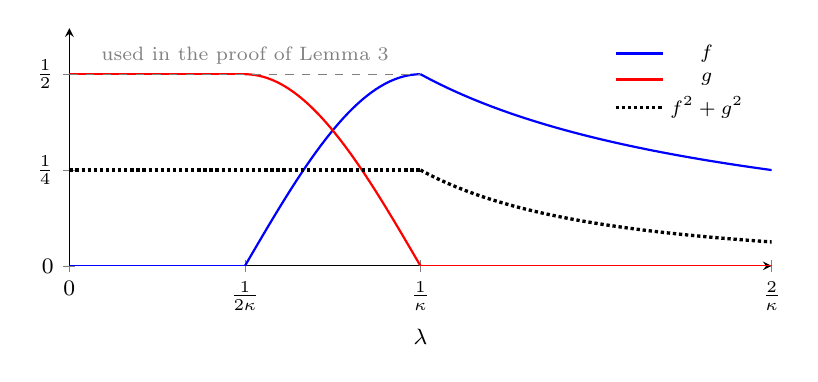
\begin{tikzpicture}
\begin{axis}[width=10.5cm, height=4.6cm, xmin=0, xmax=1, ymin=0, ymax=0.62,
  axis lines=left, xlabel={$\lambda$}, xtick={0,0.25,0.5,1}, xticklabels={$0$,$\frac1{2\kappa}$,$\frac1\kappa$,$\frac2\kappa$},
  ytick={0,0.25,0.5}, yticklabels={$0$,$\frac14$,$\frac12$}, legend style={font=\scriptsize, draw=none,
  at={(0.98,0.98)}, anchor=north east}, tick label style={font=\footnotesize}, label style={font=\footnotesize}]
\addplot[blue, thick, domain=0:0.25, forget plot] {0};
\addplot[blue, thick, domain=0.25:0.5, samples=40, forget plot] {0.5*sin(deg(pi/2*(4*x-1)))};
\addplot[blue, thick, domain=0.5:1, samples=40, forget plot] {1/(4*x)};
\addplot[red, thick, domain=0:0.25, forget plot] {0.5};
\addplot[red, thick, domain=0.25:0.5, samples=40, forget plot] {0.5*cos(deg(pi/2*(4*x-1)))};
\addplot[red, thick, domain=0.5:1, forget plot] {0};
\addplot[black, densely dotted, very thick, domain=0:0.5, forget plot] {0.25};
\addplot[black, densely dotted, very thick, domain=0.5:1, samples=40, forget plot] {1/(16*x*x)};
\addlegendimage{blue, thick}\addlegendentry{$f$}
\addlegendimage{red, thick}\addlegendentry{$g$}
\addlegendimage{black, densely dotted, very thick}\addlegendentry{$f^2+g^2$}
\addplot[gray, dashed, domain=0:0.5, forget plot] {0.5};
\node[font=\scriptsize, gray, anchor=south] at (axis cs:0.25,0.5) {used in the proof of Lemma~3};
\end{axis}
\end{tikzpicture}
\caption{The filter functions of the HHL paper for $\kappa=2$. On $[\frac1{2\kappa},\frac1\kappa)$ the
point $(f,g)$ moves on a circle of radius~$\frac12$ with angular speed $\pi\kappa$. So
$\ket{h(\lambda)}$ moves with speed exactly $\frac\pi2\kappa$ there (Lemma~2), $f^2+g^2=\frac14$ rather
than the $\frac12$ used in the paper's proof of Lemma~3, and the constant of Lemma~3 is
$\pi^2$.}\label{fig:filters}
\end{figure}

\begin{lstlisting}[float=tp,caption={The filter functions, Lemma~3 with the corrected constant, the counterexample
to the paper's constant, and sharpness (for fixed \isa{$\kappa$ > 0})},label={lst:lemma3}]
definition filt_f :: "real ~$\Rightarrow$~ real ~$\Rightarrow$~ real" where
  "filt_f ~$\kappa$~ x = (if 1 / ~$\kappa$~ ~$\le$~ x then 1 / (2 * ~$\kappa$~ * x)
                   else if 1 / (2 * ~$\kappa$~) ~$\le$~ x then sin (pi / 2 * (2 *
                       ~$\kappa$~ * x - 1)) / 2 else 0)"
definition filt_g :: "real ~$\Rightarrow$~ real ~$\Rightarrow$~ real" where
  "filt_g ~$\kappa$~ x = (if 1 / ~$\kappa$~ ~$\le$~ x then 0
                   else if 1 / (2 * ~$\kappa$~) ~$\le$~ x then cos (pi / 2 * (2 *
                       ~$\kappa$~ * x - 1)) / 2 else 1 / 2)"
theorem lemma3:
  "(filt_f ~$\kappa$~ a - filt_f ~$\kappa$~ b)~$^{2}$~ + (filt_g ~$\kappa$~ a - filt_g ~$\kappa$~ b)~$^{2}$~
     ~$\le$~ pi~$^{2}$~ * ~$\kappa^{2}$~ * (a - b)~$^{2}$~ * ((filt_f ~$\kappa$~ a)~$^{2}$~ + (filt_g ~$\kappa$~ a)~$^{2}$~)"
theorem lemma3_paper_constant:
  "pi~$^{2}$~ / 2 * ~$\kappa^{2}$~ * (1 / (2 * ~$\kappa$~) - 1 / ~$\kappa$~)~$^{2}$~ * ((filt_f ~$\kappa$~ (1 / (2 *
      ~$\kappa$~)))~$^{2}$~ + (filt_g ~$\kappa$~ (1 / (2 * ~$\kappa$~)))~$^{2}$~)
   < (filt_f ~$\kappa$~ (1 / (2 * ~$\kappa$~)) - filt_f ~$\kappa$~ (1 / ~$\kappa$~))~$^{2}$~ + (filt_g ~$\kappa$~ (1 /
       (2 * ~$\kappa$~)) - filt_g ~$\kappa$~ (1 / ~$\kappa$~))~$^{2}$~"
theorem lemma3_sharp:
  assumes c: "c < pi~$^{2}$~"
  shows "~$\exists$~a b. c * ~$\kappa^{2}$~ * (a - b)~$^{2}$~ * ((filt_f ~$\kappa$~ a)~$^{2}$~ + (filt_g ~$\kappa$~ a)~$^{2}$~)
                < (filt_f ~$\kappa$~ a - filt_f ~$\kappa$~ b)~$^{2}$~ + (filt_g ~$\kappa$~ a -
                    filt_g ~$\kappa$~ b)~$^{2}$~"
\end{lstlisting}

The counterexample is $\lambda=\frac1{2\kappa}$, $\tilde\lambda=\frac1\kappa$, where the two sides are
$\frac12$ and $\pi^2/32$. Sharpness takes both points in the middle region, where the left side is
$\sin^2(\pi\kappa(\lambda-\tilde\lambda)/2)$, and uses $\sin w\ge w-w^3/6$. The paper uses Lemma~3 for
the two error terms of the post-selected output, (A13)--(A17), and states Theorem~1 only up to
$O(\kappa/t_0)$, so the corrected constant does not change that statement.
With the corrected lemma, the window register and the wrapped distances of the grid values, all three
parts of Theorem~1 of the paper hold for every~$b$ with explicit constants. For $t=Nt_0$ the total
evolution time, $\norm{(\tilde U-U)b}\le3\pi^2\sqrt{4+2\pi^2}\,\kappa\norm b/t$, and the states
post-selected on $\{\mathit{well},\mathit{ill}\}$, or on $\mathit{well}$ when $b$ lies in the
well-conditioned subspace, are within $12\pi^2\sqrt{4+2\pi^2}\,\kappa/t$ of the ideal ones
(\isa{flag\_bound}, \isa{flag\_post\_normalized}, \isa{flag\_well\_normalized}).

\subsection{Oracles, Amplification and Run Time}

The circuit uses $e^{iAt_0}$ only through controlled powers. We model it in a small language of fixed
gates, controlled calls to an oracle $V$, and sequencing (\isa{qcirc}), with a matrix semantics
(\isa{sem}) and a call count (\isa{calls}). HHL makes $2(N-1)$ calls, and replacing the oracle by any
unitary $V$ with $\norm{Vv-e^{iAt_0}v}\le\eta\norm v$ moves the output by at most $2(N-1)\eta$, because each
call adds at most $\eta$ (\isa{hhl\_sim\_robust}). Post-selection is stable: if the output is within
$\delta$ of the exact one, the post-selected state is within $2\delta/(C\norm{A^{-1}b})$ of
$\psi\otimes A^{-1}b/\norm{A^{-1}b}\otimes\ket1$ (\isa{hhl\_readout}). Amplitude amplification is proved
in the plane spanned by the good and bad components (Fig.~\ref{fig:aa}). As a circuit, each round
uses the HHL circuit and its inverse once.

\begin{figure}[t]
\centering
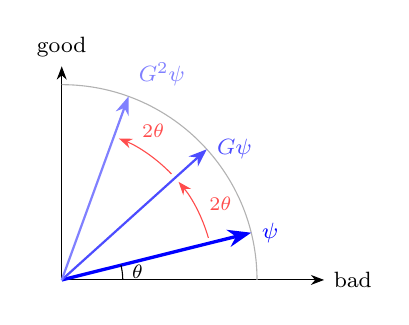
\begin{tikzpicture}[scale=1.55, >=Stealth]
\draw[->] (0,0) -- (2.15,0) node[right, font=\footnotesize] {bad};
\draw[->] (0,0) -- (0,1.75) node[above, font=\footnotesize] {good};
\draw[gray!60] (1.6,0) arc (0:90:1.6);
\draw[->, very thick, blue] (0,0) -- ({1.6*cos(14)},{1.6*sin(14)}) node[right, font=\footnotesize] {$\psi$};
\draw[->, thick, blue!70] (0,0) -- ({1.6*cos(42)},{1.6*sin(42)}) node[right, font=\footnotesize] {$G\psi$};
\draw[->, thick, blue!50] (0,0) -- ({1.6*cos(70)},{1.6*sin(70)}) node[above right, font=\footnotesize] {$G^2\psi$};
\draw (0.5,0) arc (0:14:0.5); \node[font=\scriptsize] at (0.62,0.07) {$\theta$};
\draw[->, red!70] ({1.25*cos(16)},{1.25*sin(16)}) arc (16:40:1.25); \node[font=\scriptsize, red!70] at (1.3,0.62) {$2\theta$};
\draw[->, red!70] ({1.25*cos(44)},{1.25*sin(44)}) arc (44:68:1.25); \node[font=\scriptsize, red!70] at (0.75,1.22) {$2\theta$};
\end{tikzpicture}
\caption{Amplitude amplification. The Grover iterate $G=(2\ketbra\psi\psi-I)(I-2P)$ rotates the plane
of the good component $P\psi$ and the bad component by $2\theta$, where $\sin\theta=\norm{P\psi}$. After
$k$ rounds the good amplitude is $\sin((2k+1)\theta)$: $PG^k\psi=\frac{\sin((2k+1)\theta)}{\sin\theta}P\psi$
(\isa{amplitude\_amplification}).}\label{fig:aa}
\end{figure}

The paper states its run time in a normalisation where the spectrum lies in $[1/\kappa,1]$. In that
normalisation the components combine as follows.

\begin{theorem}[run time]\label{thm:runtime}
Let the spectrum of $A$ lie in $[1/\kappa,1]$, let $t_0\le\pi/2$, $\varepsilon\kappa\le1$ and
$Nt_0\ge12\pi^2\sqrt{4+2\pi^2}\,\kappa/\varepsilon$, and let the flag gates prepare
$\ket{h(\tilde\lambda_k)}$. Then the post-selected well-conditioned output is within $\varepsilon$ of
$A^{-1}b/\norm{A^{-1}b}$, its amplitude is at least $1/(4\kappa)$, and at most $\pi\kappa$ rounds of
amplitude amplification, each with $2(N-1)$ oracle calls, succeed with probability at least
$1-\norm y^2$, where $y$ is the well-flagged part of one run.\isalink{Algorithms/HHL_Runtime.thy}{302}
\end{theorem}

\noindent\begin{minipage}{\linewidth}
\begin{lstlisting}[caption={Theorem~\ref{thm:runtime} (hypotheses abridged; \isa{out} is the output of the flag circuit
and \isa{y} its well-flagged part)},label={lst:runtime}]
theorem hhl_paper_runtime:
  assumes ... "~$\bigwedge$~l. l ~$\in$~ herm_spectrum A ~$\Longrightarrow$~ 1 / ~$\kappa$~ ~$\le$~ l ~$\wedge$~ l ~$\le$~ 1"
      and ... "0 < ~$\varepsilon$~" "~$\varepsilon$~ * ~$\kappa$~ ~$\le$~ 1" and "12 * pi~$^{2}$~ * sqrt (4 + 2 *
          pi~$^{2}$~) * ~$\kappa$~ / ~$\varepsilon$~ ~$\le$~ real N * t0"
  defines "out ~$\equiv$~ sem N (n * 3) (evolution A t0 ~$\otimes$~ 1~$_{m}$~ 3)
      (flag_full_prog N n G Prep) *~$_{v}$~ unit_vec (N * (n * 3)) 0"
  defines "y ~$\equiv$~ pflag 3 (~$\lambda$~c. c = 1) out" and "x ~$\equiv$~ herm_inv A *~$_{v}$~ b"
  shows "~$\|$~complex_of_real (1 / ~$\|$~y~$\|$~) ~$\cdot_{v}$~ y - tensor_vec (win_state
      N)
            (tensor_vec (complex_of_real (1 / ~$\|$~x~$\|$~) ~$\cdot_{v}$~ x)
                (unit_vec 3 1))~$\|$~ ~$\le$~ ~$\varepsilon$~"
    and "1 / (4 * ~$\kappa$~) ~$\le$~ ~$\|$~y~$\|$~"
    and "~$\|$~y~$\|$~ < 1 ~$\Longrightarrow$~ ~$\exists$~k. 1 - ~$\|$~y~$\|^{2}$~ ~$\le$~ ~$\|$~pflag 3 (~$\lambda$~c. c = 1) (sem
        ... (aa_prog ... k) ...)~$\|^{2}$~
           ~$\wedge$~ calls (aa_prog (N * (n * 3)) 3 (~$\lambda$~c. c = 1)
               (flag_full_prog N n G Prep) k) = (2 * k + 1) * (2 *
               (N - 1))
           ~$\wedge$~ real k ~$\le$~ pi * ~$\kappa$~"
\end{lstlisting}
\end{minipage}

Each round runs the circuit and its inverse, so the total simulated time is
$(2k+1)\cdot2(N-1)t_0=O(\kappa^2/\varepsilon)$, and the state preparation is used $O(\kappa)$ times. The
number of rounds depends on the unknown success amplitude. Following the paper, we use the
averaging lemma of Brassard, H{\o}yer, Mosca and Tapp~\cite{bhmt2002}. For $k$ uniform below
$M\ge1/\sin2\theta$, the mean of $\sin^2((2k+1)\theta)$ is at least $\frac14$ (\isa{bhmt\_quarter}). Stages
with $k$ uniform below $1,2,4,\dots$, stopped at the first success, therefore succeed with probability at
least $\frac14$ in fewer than $8\sqrt2\,\kappa$ rounds (\isa{doubling\_schedule\_kappa}).

\subsection{Inexact HHL as a Program}\label{sec:approx-programs}

The circuits of this section become gate lists with the same semantics (\isa{qgates\_sem}) and run as
programs. The post-selected state is now only close to the target, so the triples of
Theorems~\ref{thm:prog} and~\ref{thm:rus}, which assert the target exactly, become fidelity triples, the
last shape of Table~\ref{tab:readings}. For a program that initialises, runs a circuit with output
$\psi$ and measures with $M$, where $\ket t$ lies in the range of $M_1$, we prove the triple
$\hoaret{|\braket t\psi|^2I}{\mathit{prog}}{\ketbra tt}$. For the repeat-until-success loop we prove the
precondition $|\braket t\psi|^2/\norm{M_1\psi}^2$ (\isa{hoare\_prog\_overlap},
\isa{hoare\_rus\_overlap}). If the post-selected state is within $e$ of $\ket t$, the fidelity is at
least $1-e^2$.

\begin{theorem}[inexact HHL as programs]\label{thm:apxprog}
Assume the hypotheses of Theorem~\ref{thm:window} with $\norm b=1$ and $N\ge Q/\varepsilon$, a
unitary oracle $V$ with $\norm{Vv-e^{iAt_0}v}\le\eta\norm v$ and $\varepsilon+2(N-1)\eta\le Ct_0/\pi$, and
a unitary that prepares $\psi\otimes b\otimes\ket0$, where $\psi$ is the window state. Let
$e=2(\varepsilon+2(N-1)\eta)/(C\norm{A^{-1}b})$ and $\ket t=\psi\otimes A^{-1}b/\norm{A^{-1}b}\otimes\ket1$.
Then one run satisfies $\hoaret{(Ct_0/\pi)^2(1-e^2)\,I}{\mathit{prog}}{\ketbra tt}$, and the
repeat-until-success loop satisfies $\hoaret{(1-e^2)\,I}{\mathit{rus}}{\ketbra tt}$.
\end{theorem}

With $e$ from Theorem~\ref{thm:window} and the oracle bound, these are \isa{hhl\_apx\_program} and
\isa{hhl\_apx\_rus}. Amplitude amplification as a program needs at most $\pi^2/(4Ct_0)$ rounds
(\isa{hhl\_apx\_amplified}). The filtered version of Theorem~\ref{thm:runtime} gives
$\{(1-\varepsilon^2)\,I\}$ for the loop, and amplitude amplification as a program needs at most
$\pi\kappa$ rounds (\isa{hhl\_flag\_rus}, \isa{hhl\_flag\_amplified}). Table~\ref{tab:exact-inexact}
puts the exact and the inexact triples side by side.\isalink{Algorithms/HHL_Paper_Program.thy}{512}

\begin{table}[t]
\caption{HHL as programs: the triples of the exact case (Section~\ref{sec:exact}) and their inexact
counterparts (this section). In the exact column $p=C^2\norm{A^{-1}b}^2$ and the clock of $\ket t$ is
$\ket0$; in the inexact column $e$ is as in Theorem~\ref{thm:apxprog}, the clock of $\ket t$ is the
window state, and $y$ is the post-selected part of one run.}\label{tab:exact-inexact}
\centering\small
\renewcommand{\arraystretch}{1.15}
\begin{tabular}{@{}>{\raggedright\arraybackslash}p{1.9cm}>{\raggedright\arraybackslash}p{4.45cm}>{\raggedright\arraybackslash}p{5.3cm}@{}}
\toprule
& Exact & Inexact\\
\midrule
One run & $\{p\,I\}\,S\,\{P_1\}$ and $\{I\}\,S\,\{P_0+\ketbra tt\}$ &
  $\{(Ct_0/\pi)^2(1-e^2)\,I\}\,S\,\{\ketbra tt\}$\\
Repeat until success & $\{I\}\,S\,\{\ketbra tt\}$, $1/p$ rounds on average & $\{(1-e^2)\,I\}\,S\,\{\ketbra tt\}$\\
Amplified & -- & $\{(1-\norm y^2)(1-e^2)\,I\}\,S\,\{\ketbra tt\}$, at most $\pi^2/(4Ct_0)$ rounds\\
Filter functions & -- & loop $\{(1-\varepsilon^2)\,I\}$; amplified, at most $\pi\kappa$ rounds\\
\midrule
Theorems & \mbox{\isa{hhl\_success\_total}}, \mbox{\isa{hhl\_correct\_total}}, \mbox{\isa{hhl\_rus\_total}} &
  \mbox{\isa{hhl\_apx\_program}}, \mbox{\isa{hhl\_apx\_rus}}, \mbox{\isa{hhl\_apx\_amplified}},
  \mbox{\isa{hhl\_flag\_rus}}, \mbox{\isa{hhl\_flag\_amplified}}\\
\bottomrule
\end{tabular}
\end{table}

\noindent\begin{minipage}{\linewidth}
\begin{lstlisting}[caption={The repeat-until-success loop in the paper's regime (inside a context with the
hypotheses of Theorem~\ref{thm:window}, an oracle \isa{V} that is $\eta$-close to $e^{iAt_0}$ and a
preparation \isa{Prep} of the window state)},label={lst:apx}]
abbreviation (input) "apx_K ~$\equiv$~ N * (n * 2)"
abbreviation (input) "apx_O ~$\equiv$~ V ~$\otimes$~ 1~$_{m}$~ 2"
abbreviation (input) "apx_x ~$\equiv$~ herm_inv A *~$_{v}$~ b"
abbreviation (input) "apx_t ~$\equiv$~ tensor_vec (win_state N) (tensor_vec
    (complex_of_real (1 / ~$\|$~apx_x~$\|$~) ~$\cdot_{v}$~ apx_x) (unit_vec 2 1))"
abbreviation (input) "apx_e ~$\equiv$~ 2 * (~$\varepsilon$~ + 2 * real (N - 1) * ~$\eta$~) / (C
    * ~$\|$~apx_x~$\|$~)"
theorem hhl_apx_rus:
  "state_sig.hoare_total_correct [N, n, 2] (complex_of_real (1 -
      apx_e~$^{2}$~) ~$\cdot_{m}$~ 1~$_{m}$~ apx_K)
     (rus_meas apx_K (anc_proj apx_K) (qgates N (n * 2) apx_O
         (hhl_full_prog A t0 N C Prep))) (outer_prod apx_t apx_t)"
\end{lstlisting}
\end{minipage}
\section{Down to Elementary Gates}\label{sec:gates}

The programs of Sections~\ref{sec:exact} and~\ref{sec:approx} use large gates: $H^{\otimes k}$, the
controlled powers $\Lambda(U)$, $F_N$, the rotation stage, the preparations of $\ket b$ and of the clock,
and the oracle $e^{iAt_0}$. A gate is \emph{elementary} if it is a one- or two-qubit unitary acting on
adjacent wires, $I_a\otimes G\otimes I_b$ with $G$ a $2\times2$ or $4\times4$ unitary
(Listing~\ref{lst:elem}). This section replaces every large gate by elementary ones. Each refinement
proves that the product of the new gates equals the old gate, so every triple carries over
(Section~\ref{sec:qhl}).

\subsection{The Gate-Level Circuit}

The Hadamard layer is $k$ single-qubit Hadamards. The controlled powers factor over the clock bits,
$\Lambda(U)=\prod_jC_j(U^{2^j})$, where $C_j$ is controlled by bit~$j$ of the clock
(\isa{ctrl\_pow\_qubits}). Equivalently, they use $2^k-1$ singly controlled copies of~$U$
(\isa{ctrl\_pow\_queries}). The Fourier transform is the AFP's gate-level circuit, flattened into
Hadamards, controlled phase rotations and swaps (\isa{qft\_circuit}). It has $(k^3+2k)/3$ gates, which
is cubic because its controlled rotations are routed through nearest-neighbour swaps. The resulting
circuit for HHL has $(2k^3+16k+6)/3$ gates (\isa{length\_hhl\_elem\_gates}), and every gate is
elementary except the oracle calls $C_j(U^{\pm2^j})$, the preparation $U_b$ and the rotation stage
(\isa{hhl\_elem\_gate\_kinds}).\isalink{Algorithms/HHL_Gates.thy}{84}

\noindent\begin{minipage}{\linewidth}
\begin{lstlisting}[caption={Elementary gates, the Fourier circuit, and the gate count},label={lst:elem}]
definition elementary :: "nat ~$\Rightarrow$~ complex mat ~$\Rightarrow$~ bool" where
  "elementary K U ~$\longleftrightarrow$~ (~$\exists$~a b q G. q ~$\in$~ {1, 2} ~$\wedge$~ G ~$\in$~ carrier_mat (2 ^
      q) (2 ^ q) ~$\wedge$~ unitary G ~$\wedge$~ 0 < a ~$\wedge$~ 0 < b ~$\wedge$~
     K = a * (2 ^ q * b) ~$\wedge$~ U = 1~$_{m}$~ a ~$\otimes$~ (G ~$\otimes$~ 1~$_{m}$~ b))"
theorem qft_circuit:
  shows "circuit_mat (2 ^ n) (qft_circuit n) = fourier (2 ^ n)"
    and "U ~$\in$~ set (qft_circuit n) ~$\Longrightarrow$~ elementary (2 ^ n) U"
theorem length_hhl_elem_gates: "3 * length (hhl_elem_gates A Ub t0
    k C) = 2 * k ^ 3 + 16 * k + 6"
\end{lstlisting}
\end{minipage}

\subsection{The Rotation as a Uniformly Controlled Rotation}

The rotation stage $\sum_c\ketbra cc\otimes I\otimes\mathrm{Rot}(\theta_c)$, with $\theta_c=\arcsin(C/\lambda_c)$
and $\mathrm{Rot}(a)$ the real rotation by~$a$, applies a different angle for each of the $2^k$ clock
values. Write the angles in the Walsh--Hadamard basis,
$\theta_c=\sum_{S\subseteq\{0,\dots,k-1\}}w_S(-1)^{\pi_S(c)}$, where $\pi_S(c)$ is the parity of the bits
of~$c$ in~$S$ and $w_S=2^{-k}\sum_{c'}\theta_{c'}(-1)^{\pi_S(c')}$ (\isa{walsh\_inversion}). Then the
stage is one rotation of the ancilla by $\sum_Sw_S$, followed by one block per non-empty $S$. A block
computes $\pi_S(c)$ into the last clock qubit with a chain of nearest-neighbour CNOT and SWAP gates,
rotates the ancilla by $-2w_S$ controlled by that qubit, and uncomputes the chain
(Fig.~\ref{fig:ucr}a, \isa{ucr\_circuit}). For a system register of $s$ qubits, the controlled rotation
is moved next to the clock by $s$ adjacent swaps (\isa{route\_cv0}).\isalink{Algorithms/HHL_Uniform_Rotation.thy}{691}

\begin{figure}[t]
\centering
\textbf{(a)}\quad
\scalebox{0.8}{%
\begin{quantikz}[row sep={0.62cm,between origins}, column sep=0.25cm]
\lstick{$c_2$} & & \swap{1} & & & & \swap{1} & \midstick[5,brackets=none]{$\cdots$} & \\
\lstick{$c_1$} & & \targX{} & \ctrl{1} & & \ctrl{1} & \targX{} & & \\
\lstick{$c_0$} & & & \targ{} & \ctrl{2} & \targ{} & & & \\
\lstick{system} & \qwbundle{s} & & & & & & & \\
\lstick{ancilla} & \gate{\mathrm{Rot}(\textstyle\sum_Sw_S)} & & & \gate{\mathrm{Rot}(-2w_{\{0,2\}})} & & & &
\end{quantikz}}
\\[0.5em]
\textbf{(b)}\quad
\scalebox{0.8}{%
\begin{quantikz}[row sep={0.62cm,between origins}, column sep=0.3cm]
\lstick{$q_0$} & \gate{\mathrm{Rot}(a_{\varepsilon})} & \gate[2]{\mathrm{UCR}} & \gate[3]{\mathrm{UCR}} & \gate[3]{D_\phi} & \rstick[3]{$b$}\\
\lstick{$q_1$} & & & & & \\
\lstick{$q_2$} & & & & &
\end{quantikz}}
\caption{(a) One block of the uniformly controlled rotation for $k=3$ and $S=\{0,2\}$: the SWAP and
CNOT put $c_0\oplus c_2$ into $c_0$, a rotation of the ancilla controlled by $c_0$ follows, and the chain
is undone. The ancilla rotation controlled by $c_0$ crosses the system register, and is routed by
adjacent swaps. (b) State preparation on three qubits. Level $j$ rotates qubit $j$ by an angle that
depends on the qubits before it, $a_c=\arcsin(\norm{b_{c1}}/\norm{b_c})$ for the blocks $b_c$ of $b$
indexed by the prefix~$c$, as a uniformly controlled rotation; a diagonal unitary $D_\phi$ then sets
the phases.}\label{fig:ucr}
\end{figure}

\noindent\begin{minipage}{\linewidth}
\begin{lstlisting}[caption={The rotation stage as a uniformly controlled rotation},label={lst:ucr}]
theorem ucr_circuit:
  assumes n0: "0 < n"
  shows "circuit_mat (2 ^ k * (n * 2)) (ucr_gates k n ~$\theta$~) =
      ctrl_blocks (2 ^ k) (n * 2) (~$\lambda$~c. 1~$_{m}$~ n ~$\otimes$~ Rot (~$\theta$~ c))"
theorem ucr_gate_kinds:
  assumes U: "U ~$\in$~ set (ucr_gates k n ~$\theta$~)" and n0: "0 < n"
  shows "elementary (2 ^ k * (n * 2)) U ~$\vee$~ (~$\exists$~a. U = cv0 k n (Rot
      a))"
\end{lstlisting}
\end{minipage}

\subsection{State Preparation}

A state with non-negative amplitudes $a$ on $k$ qubits is prepared by $k$ levels of uniformly controlled
rotations, the construction of Grover and Rudolph~\cite{groverrudolph2002} and M\"ott\"onen et
al.~\cite{mottonen2005}. Level $j$ rotates qubit $j$ by the angle $\arcsin(\norm{a_{c1}}/\norm{a_c})$
determined by the block norms (\isa{cascade\_prepares}, \isa{state\_prep}). The sine window is one
instance (\isa{window\_prep}). For a complex $b$, the magnitudes are prepared first and the phases are
set by a diagonal unitary. A diagonal unitary on $k+1$ qubits splits into a diagonal unitary on $k$
qubits, carrying the means of the phases of each pair, and a uniformly controlled rotation conjugated by
a fixed one-qubit gate, carrying their differences (\isa{diag\_gates\_circuit}). This yields the
following theorem.\isalink{Algorithms/HHL_All_Elementary.thy}{444}

\noindent\begin{minipage}{\linewidth}
\begin{lstlisting}[caption={Every normalised $\ket b$ is prepared by elementary gates},label={lst:bprep}]
theorem bprep:
  assumes s: "1 ~$\le$~ s" and b: "dim_vec b = 2 ^ s" "~$\|$~b~$\|$~ = 1"
  shows "circuit_mat (2 ^ s) (bprep_gates s b) *~$_{v}$~ unit_vec (2 ^ s)
      0 = b"
    and "~$\bigwedge$~U. U ~$\in$~ set (bprep_gates s b) ~$\Longrightarrow$~ elementary (2 ^ s) U"
    and "circuit_mat (2 ^ s) (bprep_gates s b) ~$\in$~ carrier_mat (2 ^
        s) (2 ^ s)"
    and "unitary (circuit_mat (2 ^ s) (bprep_gates s b))"
\end{lstlisting}
\end{minipage}

\subsection{Every Gate Elementary}

For $n=2^s$, the refinements combine into the program \isa{hhl\_elementary}: it satisfies the three
triples of Theorems~\ref{thm:prog} and~\ref{thm:rus}, and every gate is elementary or an oracle call
$C_j(U^{\pm2^j})$. The same holds for the paper-regime programs of
Section~\ref{sec:approx-programs} (\isa{hhl\_apx\_elementary}), where the oracle is the approximate
evolution~$V$. The oracle calls themselves can be compiled. By the spectral theorem for normal matrices
(taken from QHLProver), every unitary is $U=\prod_k(I+(\lambda_k-1)p_kp_k^\dagger)$ for an orthonormal
eigenbasis $(p_k)$. Each factor is $Q_kD_kQ_k^\dagger$, where $Q_k$ is the preparation circuit of $p_k$
and $D_k$ multiplies $\ket0$ by the phase~$\lambda_k$. This gives exact universality, and hence HHL
programs in which every gate is elementary.\isalink{Algorithms/HHL_All_Elementary.thy}{804}

\noindent\begin{minipage}{\linewidth}
\begin{lstlisting}[caption={Exact universality, and HHL with every gate elementary (the triples are those of
Listings~\ref{lst:progthm} and~\ref{lst:rus}; hypotheses as there, with $n=2^s$ and $\norm b=1$)},label={lst:univ}]
theorem exact_universality:
  assumes U: "U ~$\in$~ carrier_mat (2 ^ m) (2 ^ m)" "unitary U" and m:
      "1 ~$\le$~ m"
  shows "~$\exists$~Gs. (~$\forall$~G ~$\in$~ set Gs. elementary (2 ^ m) G) ~$\wedge$~ circuit_mat (2
      ^ m) Gs = U"
theorem hhl_compiled:
  assumes ...
  defines "K ~$\equiv$~ 2 ^ k * (2 ^ s * 2)"
  shows "~$\exists$~Gs. (~$\forall$~G ~$\in$~ set Gs. elementary K G)
     ~$\wedge$~ state_sig.hoare_total_correct [2 ^ k, 2 ^ s, 2]
         (complex_of_real (C~$^{2}$~ * ~$\|$~herm_inv A *~$_{v}$~ b~$\|^{2}$~) ~$\cdot_{m}$~ 1~$_{m}$~ K)
           (hhl_prog K Gs) (anc_proj K 1)
     ~$\wedge$~ state_sig.hoare_total_correct [2 ^ k, 2 ^ s, 2] (1~$_{m}$~ K)
         (hhl_prog K Gs)
           (anc_proj K 0 + outer_prod (hhl_target A k b)
               (hhl_target A k b))
     ~$\wedge$~ (C ~$\neq$~ 0 ~$\longrightarrow$~ state_sig.hoare_total_correct [2 ^ k, 2 ^ s, 2]
         (1~$_{m}$~ K) (hhl_rus_prog K Gs)
           (outer_prod (hhl_target A k b) (hhl_target A k b)))"
\end{lstlisting}
\end{minipage}

Universality comes with no useful bound on the number of gates, so for cost statements the oracle
calls remain the unit of measure. When $A$ is sparse, a better circuit for the oracle exists.

\subsection{Sparse Hamiltonian Simulation}

The paper assumes $s$-sparse $A$ and cites simulation results for $e^{iAt}$~\cite{berry2007}. We
formalise the first-order version of this construction in three steps.

\paragraph{Trotter.} For Hermitian $H_1,\dots,H_m$ with $\norm{H_j}\le L$,
\[
\bigl\|(e^{itH_1/r}\cdots e^{itH_m/r})^r-e^{it(H_1+\dots+H_m)}\bigr\|\le2(mLt)^2/r
\]
(\isa{trotter}, Listing~\ref{lst:sparse}). The proof stays in the functional calculus.
$|e^{ix}-1-ix|\le x^2$ bounds each factor to first order, and the errors add along products and powers of
unitaries.

\paragraph{Colouring.} The graph of an $s$-sparse Hermitian $A$ is edge-coloured greedily with $2s-1$
colours. Each colour class is a matching, given by an involution $q_c$ of the index set, so $A$ is its
diagonal plus $2s-1$ Hermitian 1-sparse matrices whose entries are entries of~$A$
(\isa{sparse\_split})~\cite{aharonov2003,berry2007}.

\paragraph{The 1-sparse circuit.} Each 1-sparse evolution is implemented exactly on
$\ket x\ket y\ket b$ (Fig.~\ref{fig:sparse}). A colour oracle $O_c$ writes the partner $q_c(x)$ into the
second register. A comparator sorts the pair and records the order in~$b$. An entry gate rotates $b$
by $e^{id\left(\begin{smallmatrix}0&a\\\bar a&0\end{smallmatrix}\right)}$ with $a=A_{xy}$. The comparator and
$O_c^\dagger$ then uncompute (\isa{colour\_circ\_basis}). The oracle is a hypothesis, any unitary with
$\ket x\ket0\ket b\mapsto\ket x\ket{q_c(x)}\ket b$, and one exists for every colouring. A final gate
applies the phases of the diagonal.\isalink{Algorithms/HHL_Sparse_Circuit.thy}{914}

\begin{figure}[t]
\centering
\scalebox{0.85}{%
\begin{quantikz}[row sep={0.7cm,between origins}, column sep=0.3cm]
\lstick{$\ket x$} & \qwbundle{} & \gate[2]{O_c} & \gate[3]{\mathrm{CMP}} & \gate[3]{\mathrm{ENT}_d} & \gate[3]{\mathrm{CMP}} & \gate[2]{O_c^\dagger} & \midstick[3,brackets=none]{$\cdots$} & \gate{D_d} & \rstick{$V_d\ket x$}\\
\lstick{$\ket 0$} & \qwbundle{} & & & & & & & & \rstick{$\ket0$}\\
\lstick{$\ket 0$} & & & & & & & & & \rstick{$\ket0$}
\end{quantikz}}
\caption{One Trotter step for an $s$-sparse $A$ with $d=t/r$. For each of the $2s-1$ colours~$c$, five
gates implement $e^{idH_c}$ on $\ket x$ with both ancilla registers returned to $\ket0$, where $H_c$ is
the 1-sparse part of colour $c$. A diagonal phase gate $D_d=e^{id\operatorname{diag}A}$ follows, so the
step acts on $\ket x$ as the product $V_d$ of the $2s$ part evolutions. It has $5(2s-1)+1$ gates, and
$r$ steps use $r(6s-2)$ oracle queries.}\label{fig:sparse}
\end{figure}

\begin{lstlisting}[float=tp,caption={Trotter, the colouring, and the sparse simulation circuit},label={lst:sparse}]
theorem trotter:
  assumes Hs: "~$\bigwedge$~H. H ~$\in$~ set Hs ~$\Longrightarrow$~ herm_bounded n L H" and r: "0 < r"
  shows "op_close n (2 * (real (length Hs) * L * t)~$^{2}$~ / real r)
           (tprod n (t / real r) Hs ^~$_{m}$~ r) (evolution (hsum n Hs)
               t)"
theorem sparse_split:
  assumes A: "A ~$\in$~ carrier_mat n n" "hermitian A" and sp: "sparse n
      s A" and s: "1 ~$\le$~ s"
  shows "~$\exists$~p. edge_cover n (2 * s - 1) p (edges n A) ~$\wedge$~
           length (sparse_parts n A (2 * s - 1) p) = 2 * s ~$\wedge$~ hsum
               n (sparse_parts n A (2 * s - 1) p) = A"
theorem sparse_simulation_circuit:
  assumes A: "A ~$\in$~ carrier_mat n n" "hermitian A" and s: "1 ~$\le$~ s"
      and L: "0 ~$\le$~ L" and Lb: "~$\bigwedge$~i j. i < n ~$\Longrightarrow$~ j < n ~$\Longrightarrow$~ cmod (A ~\$\$~ (i,
          j)) ~$\le$~ L"
      and cov: "edge_cover n (2 * s - 1) p (edges n A)"
      and Os: "~$\bigwedge$~c. c < 2 * s - 1 ~$\Longrightarrow$~ colour_oracle n (p c) (Os c)"
          and r: "0 < r"
  shows "sg_run n (t / real r) A Os (sim_gates (2 * s - 1) r) *
      emb n = emb n * sim_mat n (t / real r) A (2 * s - 1) p r"
    and "sim_mat n (t / real r) A (2 * s - 1) p r ~$\in$~ carrier_mat n
        n"
    and "unitary (sim_mat n (t / real r) A (2 * s - 1) p r)"
    and "op_close n (8 * (real s * L * t)~$^{2}$~ / real r) (sim_mat n (t
        / real r) A (2 * s - 1) p r) (evolution A t)"
    and "length (filter is_query (sim_gates (2 * s - 1) r)) = r *
        (6 * s - 2)"
\end{lstlisting}

The circuit acts on inputs with both ancilla registers zero as a unitary $V$ on the system
(\isa{emb} embeds the system). $V$ is within $8(sLt)^2/r$ of $e^{itA}$, where $L$ bounds the entries of~$A$.
Plugged into the error bound of Section~\ref{sec:approx}, this gives the output error
$(\varepsilon+16(N-1)(sLt_0)^2/r)\norm b$ (\isa{hhl\_sparse\_window\_error}). The higher-order formulas
behind the paper's cited cost, and the reversible arithmetic inside the oracles, are not formalised.
\section{What the Formalisation Found}\label{sec:errata}

The HHL paper is a carefully written letter with a long appendix, and its main claims survive
mechanisation. Its details do not all survive. Table~\ref{tab:errata} lists the statements of the
arXiv version~\cite{hhl2008arxiv} that are false as written, with the correction and its formal witness.
Most errors are in the appendix on the optimality of the algorithm, which reduces quantum circuits to
matrix inversion (Theorems~4--6). Each optimality theorem is formalised up to the external
complexity-theoretic fact it cites (PSPACE-completeness of TQBF, $\mathrm{BQP}\subseteq\mathrm{PSPACE}$,
and the classical lower bounds for Simon's problem and parity). The search lower bound of Theorem~4(2)
is imported from the AFP entry \emph{Compressed Oracles}.

\begin{table}[t]
\caption{Errata in the HHL paper (arXiv:0811.3171v3). ``Formal'' names the theorem that refutes the claim
or proves the correction.}\label{tab:errata}
\centering\scriptsize
\renewcommand{\arraystretch}{1.12}
\newcolumntype{L}[1]{>{\raggedright\arraybackslash}p{#1}}
\begin{tabular}{@{}L{1.3cm}L{2.75cm}L{4.35cm}L{2.75cm}@{}}
\toprule
Where & Claim & Correction & Formal\\
\midrule
Lemma 3 & $c=\pi^2/2$ & false for every $\kappa$ (at $\lambda=\frac1{2\kappa}$, $\tilde\lambda=\frac1\kappa$); $c=\pi^2$ holds and is sharp & \isa{lemma3\_paper\_constant}, \isa{lemma3}, \isa{lemma3\_sharp}\\
Proof of Thm.~4 & $m=\frac2\delta\log(2n)/\log\log n$ rounds suffice & too few: for $n_0=2^{64}$, $\delta=\frac12$ it gives $m=130/3$, and after $m\le44$ rounds the bound on $T_m$ still exceeds $n_0$; $m\ge\frac2\delta\ln(2n_0)$ suffices & \isa{paper\_rounds\_insufficient}, \isa{corrected\_rounds}\\
(A34) & the dilation satisfies $\kappa^{-1}I\le A\le I$ & impossible: its diagonal is zero & \isa{herm\_embed\_diag}\\
(A37) & the first qubit of $\vec y$ decides acceptance & the top half of $\vec y$ is always $0$; permuting the dilation fixes it & \isa{first\_half\_perm}, \isa{red\_first\_qubit}\\
Thm.~6(2) & precision $\varepsilon=2^{-n-2}$ & cannot separate counts $C$ and $C+1$ once the clock factor ($\le\frac14$) is included & \isa{paper\_precision\_insufficient}\\
App.~A5 & $1/(3\varepsilon^2)$ samples & too few: $\varepsilon=\frac14$, $p=\frac12$ and $6$ samples fail with probability $\frac{11}{16}$; $3/\varepsilon^2$ suffice & \isa{paper\_sample\_count\_too\_small}, \isa{estimate\_expectation}\\
\S IV & preconditioned system $(AB)c=Bb$ & neither left nor right preconditioning: in a $2\times2$ example its unique solution gives no solution of $Ax=b$ & \isa{paper\_precondition\_wrong}\\
App.~A5 & undo gates $U^\dagger_{3T+1-t}$ & must be $U^\dagger_{T+1-t}$ & construction \isa{red\_U}, \isa{red\_inverse}\\
App.~A5 & $\kappa\le2T$ & $\kappa=\coth\frac1{2T}>2T$ when $3T$ is even (not formalised); we prove $\kappa\le2T+1$ & \isa{red\_A\_bounds}\\
\bottomrule
\end{tabular}
\end{table}

The last two rows are corrections built into the formal construction rather than refutations: the
reduction is defined with the correct undo gates, and only the weaker bound $2T+1$ is proved. The other
rows are refuted by explicit counterexamples. Three observations are worth recording. First, none of
the errors we found invalidates a main claim of the paper: those are stated with $O(\cdot)$ and survive
with other constants.
Second, the errors sit where a proof sketch compresses a computation, for instance an evaluation of
$f^2+g^2$, an index, or a number of rounds. Third, a recent re-derivation of the error
analysis~\cite{liphillips2024} remarks that the factor $\pi/2$ of Lemma~2 ``is not correct for certain
values of~$\kappa$''. With the paper's choice $\kappa'=2\kappa$, which places the middle region at $[\frac1{2\kappa},\frac1\kappa)$,
our proof \isa{hflag\_lipschitz} shows that $\lambda\mapsto\ket{h(\lambda)}$ is
$\frac\pi2\kappa$-Lipschitz for every $\kappa>0$, so Lemma~2 is correct as stated. A machine-checked
proof settles such disagreements.

The lecture notes of Section~\ref{sec:paulsen} also contain false statements, all found because a
statement failed to be provable as written. The Day~29 ``Hamming $[7,1,3]$'' code has distance $2$ and
cannot correct one error (\isa{notes\_hamming\_not\_correcting}). The Day~32 claim that distinct
one-qubit Pauli errors map the Shor code to orthogonal subspaces fails for $Z_1\neq Z_2$, which agree on
the code space (\isa{shor\_notes\_Z1\_Z2}; the notes correct it on Day~33). A reformulation of the Day~21
conjecture is false for $n=2$, $d=1$ (\isa{notes\_form\_i\_false}). Two Day~23 examples, a formula of
Day~31 and Cholesky's reduction on Day~5 each need an extra hypothesis.
\section{The Foundation: Paulsen's Lectures, Formalised}\label{sec:paulsen}

The HHL development builds on a formalisation of one complete set of lecture notes: Vern Paulsen's
\emph{Lectures on Quantum Computing and Completely Positive Maps} (Houston, 2011)~\cite{paulsen2011notes}.
The notes are an unedited transcription of 34 lectures in five parts: basic mathematics, an introduction
to quantum computing, completely positive maps, entanglement, and error correction. Taking a course as
the specification forces one to formalise the whole supporting theory rather than the shortest path to
a headline theorem. It also gives an external measure of completeness.

\paragraph{Audit and document.} The repository's audit lists every definition, theorem, proposition,
corollary, example and remark of the notes with its formal counterpart. Of the 170 items, 9 are
deliberately not formalised (overviews, history, classical asides). Of the remaining 161, 156 are
formalised faithfully, 5 in a variant form, and none is missing. The variants are a different proof
route (Choi's Theorem~3 through a Radon--Nikodym theorem for completely positive maps, and Arveson's
extension theorem by cone separation), or a statement of the notes that needs a hypothesis or is false
(Section~\ref{sec:errata}). The HHL paper is audited in the same way, in 23 items. An Isabelle-generated
document of 404 pages restates the notes lecture by lecture, with the formal statements in place of the
informal proofs, and it is rebuilt and re-checked by every build.

\paragraph{Contents.} Lectures 1--10 give the linear algebra and the postulates: Schur's theorem, the
spectral theorem, four characterisations of positivity, Cholesky's reduction, tensor products,
measurements and POVMs. Part VI imports exactly this part. Lectures 11--22 give density matrices,
partial traces, and completely positive maps with Choi's theorem (Listing~\ref{lst:choi}) and the
Choi--Kraus representation. Lectures 23--28 give the extreme points of the unital and of the
trace-preserving channels (Choi's Theorem~3), the Hahn--Banach theorem on matrix spaces, Arveson's
extension theorem, and the separating-hyperplane theory of entanglement witnesses. Lectures 29--34 give
classical and quantum codes, the Knill--Laflamme conditions in both directions, and Shor's nine-qubit
code. One CPTP map corrects every single-qubit unitary error on each of the nine qubits
(\isa{shor\_code\_theorem}); the $2^9$-dimensional space is never handled entrywise but as three blocks of
three qubits.\isalink{Day11/Quantum_Computing11.thy}{6486}

\noindent\begin{minipage}{\linewidth}
\begin{lstlisting}[caption={Choi's theorem (Lecture 19)},label={lst:choi}]
theorem choi_theorem:
  fixes ~$\Phi$~ :: "complex mat ~$\Rightarrow$~ complex mat"
  assumes linear: "~$\bigwedge$~A B. A ~$\in$~ carrier_mat n n ~$\Longrightarrow$~ B ~$\in$~ carrier_mat n n
      ~$\Longrightarrow$~ ~$\Phi$~ (A + B) = ~$\Phi$~ A + ~$\Phi$~ B"
      and smult: "~$\bigwedge$~c A. A ~$\in$~ carrier_mat n n ~$\Longrightarrow$~ ~$\Phi$~ (c ~$\cdot_{m}$~ A) = c ~$\cdot_{m}$~ ~$\Phi$~ A"
      and range: "~$\forall$~A. A ~$\in$~ carrier_mat n n ~$\longrightarrow$~ ~$\Phi$~ A ~$\in$~ carrier_mat d d"
      and npos: "n > 0" and dpos: "d > 0"
  shows "completely_positive n d ~$\Phi$~ ~$\longleftrightarrow$~ psd (choi_matrix n d ~$\Phi$~)"
\end{lstlisting}
\end{minipage}

\paragraph{Two lessons.} First, HOL functions are total, while a map $M_n\to M_d$ is constrained only on
the carrier. The naive definition of an extreme point (``$\Phi$ is not the midpoint of two different
channels'') is therefore vacuous, since any channel agrees on the carrier with maps that differ from it
elsewhere. Extremality has to be defined through disagreement on the carrier. Second, two places in the
notes genuinely need topology: the compactness of the unital channels, and the separation of a point
from the closed convex cone of separable matrices. For these we wrap matrices of fixed dimension in a
type, instantiate HOL-Analysis up to \isa{euclidean\_space}, and transport the statements back. The
carrier-predicate world carries almost all of the development, and the typed world is used only where
HOL-Analysis is applied.

\paragraph{An open problem.} Lecture~21 asks whether every unital completely positive map
$\Phi:M_n\to M_d$ is the average of $n$ unital maps of Choi rank at most~$d$. This is the strong
Ruskai--Audenaert conjecture for the dual channel, which is open in general~\cite{kumarwolf2026}. We state
it formally (\isa{D21\_2}) and prove the cases with direct constructions. If the Kraus operators split
into $n$ groups that are orthogonal in a suitable sense, Fourier mixtures give the decomposition
(\isa{fourier\_split}). This covers measurement maps and, via Horn's lemma, the case $d=1$. Following
Bacon, Smolin and Wolf, every unital map with $n=2$ is such an average (\isa{ra\_two}): the off-diagonal
block of the Choi matrix is $R_1KR_2^\dagger$ for a contraction $K$, and $K=\frac12(U_1+U_2)$ for unitaries
obtained from a singular value decomposition, which we build from the spectral theorem. A
reformulation in the notes turned out to be false (Section~\ref{sec:errata}).

\paragraph{Size.} The formalisation of the notes has 50 theories with 51\,729 lines and 1\,614 results
(lemmas, theorems, corollaries and propositions). Part VI has 31 theories with 21\,414 lines and 1\,087
results, plus an 80-line bridge to the AFP's quantum search bound in a separate session
(Table~\ref{tab:stats}).
\section{Related Work}\label{sec:related}

\paragraph{Verified HHL.} Zhou, Yu and Ying introduced an applied quantum Hoare logic with projection
predicates and rules for robustness, and used it for a pen-and-paper verification of
HHL~\cite{zhou2019applied}. CoqQ~\cite{zhou2023coqq} formalised that proof in Coq. Under the assumption
that every $\lambda_jt_0/2\pi$ lies in $\{1,\dots,N-1\}$, it proves $\hoarep{I}{\mathit{HHL}}{\ketbra xx}$
for the repeat-until-success program, in about 280 lines. $U_b$ and the controlled rotation are built
from partial specifications, and the controlled evolution is a built-in multiplexer. Wu, Deng and Xu~\cite{wu2024local} verify the
same exact HHL, and Shor's algorithm, in a quantum Hoare logic with distribution formulas embedded in
Coq. Our development is in Isabelle/HOL and differs in scope. It proves total correctness, including
termination and the distribution of the number of rounds; it treats the regime of the paper's error
analysis, with inexact eigenvalues, an approximate oracle, the filter functions and amplitude
amplification; it compiles the programs to elementary gates and simulates sparse Hamiltonians; and it
records the errata of Section~\ref{sec:errata}.

\paragraph{Other verified quantum algorithms.} In Coq, SQIR and its applications verify phase
estimation, Grover's algorithm and others~\cite{hietala2021sqir}, and an end-to-end implementation of
Shor's algorithm, including the reversible arithmetic of modular exponentiation~\cite{peng2023shor}. In
Why3, QBricks verifies phase estimation, Grover's algorithm and the order-finding part of Shor's
algorithm~\cite{chareton2021qbricks}. Besides the $4/\pi^2$ bound, our phase-estimation results include the tail
bound and the number of clock qubits of Nielsen and Chuang, stated as triples with exact weakest
preconditions. A recent HOL Light development treats Grover's
algorithm~\cite{sun2026grover}. In Isabelle, \IMD{} formalises qubits, gates, teleportation, the no-cloning
theorem and the Deutsch--Jozsa algorithm~\cite{bordg2021imd,bordg2020afp}. QHLProver verifies Grover's
algorithm with the logic we use~\cite{liu2019qhl}, and the AFP contains the quantum Fourier
transform~\cite{manrique2025qft}. Unruh's libraries develop bounded operators, tensor products of Hilbert
spaces and Kraus maps in infinite dimension~\cite{caballero2021cbo,unruh2024tensor,unruh2025kraus}; they
underlie his quantum relational Hoare logic~\cite{unruh2019qrhl} and the compressed-oracle technique,
whose search lower bound~\cite{unruh2025co} we import for Theorem~4(2) of the HHL paper. We also import
Sylvester's criterion from the AFP~\cite{binder2024hermitian}.

\paragraph{Error analyses of HHL.} Li and Phillips~\cite{liphillips2024} re-derive the paper's error
analysis by hand, with corrections of typos and with more detail on the amplitudes after phase
estimation. Their remark on Lemma~2 is discussed in Section~\ref{sec:errata}. The later literature
improves the dependence on $\kappa$ and $\varepsilon$~\cite{childs2017}. Verifying those algorithms is
future work.

\section{Discussion}\label{sec:discussion}

\paragraph{What is trusted.} Beyond Isabelle's kernel, the statements depend on the definitions they
use. Those of the AFP entries Jordan-Normal-Form, \IMD{} and QHLProver fix matrices, gates, programs,
their semantics and the meaning of triples. Our own definitions are the ones shown in the listings: the
grid values \isa{reg\_eig}, the functional calculus, the eight gates and the programs, the filter
functions, the predicate \isa{elementary}, and the colour oracle. A reader who accepts the listings and
the AFP's semantics can check that the theorems say what this paper claims.

\paragraph{Assumptions and limitations.} The preparation of $\ket b$ is a hypothesis
($U_b\ket0=b$) in Sections~\ref{sec:exact}--\ref{sec:approx} and a circuit in Section~\ref{sec:gates}. The
colour oracles of the sparse simulation are hypotheses about their action on basis states. The
reversible arithmetic that would implement them, and the higher-order product formulas behind the
paper's cost, are not formalised. Universality is exact but gives no gate count, and the routing of the
controlled rotation assumes $n=2^s$. Costs are stated as numbers of gates, oracle calls and rounds,
not as membership in complexity classes. The optimality theorems are formalised up to the
complexity-theoretic facts they cite.

\begin{table}[t]
\caption{Size of the development (results are lemmas, theorems, corollaries and propositions).}\label{tab:stats}
\centering\small
\begin{tabular}{@{}l@{\qquad}r@{\quad}r@{\quad}r@{}}
\toprule
Part & Theories & Lines & Results\\
\midrule
Mathematics (functional calculus, phase estimation) & 5 & 1\,515 & 94\\
Algorithm (circuits, error analysis, rest of the paper) & 13 & 10\,320 & 496\\
Program (QHLProver programs and triples) & 6 & 3\,768 & 185\\
Circuit (elementary gates, sparse simulation) & 7 & 5\,811 & 312\\
\midrule
Part VI, HHL & 31 & 21\,414 & 1\,087\\
Bridge to the AFP search bound (separate session) & 1 & 80 & 4\\
The example run of Section~\ref{sec:run} (separate session) & 1 & 313 & 34\\
Paulsen's lectures (the foundation) & 50 & 51\,729 & 1\,614\\
\bottomrule
\end{tabular}
\end{table}

\paragraph{Lessons.} Four proof patterns carried most of the work. First, statements about every
right-hand side are proved for eigenvectors and extended by the lemma that matrices agreeing on all
eigenvectors are equal, so no sum over an eigenbasis appears. Second, register sums
$\sum_j\ket j\otimes f_j$ make block-diagonal operators act branch by branch, which turns the error analysis
into scalar estimates. Third, every triple is proved for all gate lists with a given product, so each
refinement towards elementary gates is a circuit identity with no new program reasoning. Fourth, the
total correctness of repeat-until-success loops reduces to a geometric series once the body resets the
state. On the side of the tools, an oracle audit (\isa{Thm\_Deps.all\_oracles}) is meaningful only for
builds with \texttt{quick\_and\_dirty = false}. With \texttt{quick\_and\_dirty = true}, Isabelle discharges
internal goals of the \isa{fun} and \isa{record} packages by \isa{Skip\_Proof.cheat\_tac}, and every theorem downstream
of such a definition reports the oracle \isa{skip\_proof}, even in a development without a single
\texttt{sorry}.

\section{Conclusion}\label{sec:conclusion}

We have verified the HHL algorithm in Isabelle/HOL as programs of a quantum while-language, with
quantum Hoare logic as the common language from the functional calculus up to elementary gates. Phase
estimation, its core, is verified as a program with exact weakest preconditions, from which the
textbook guarantees, including the clock size for a given precision and confidence, follow as triples.
In the exact case the HHL program is totally correct: it succeeds with probability
$C^2\norm{A^{-1}b}^2$, it is exact on success, and its repeat-until-success loop terminates with
probability one after $1/p$ expected rounds. In the inexact case, the regime of the paper's error
analysis, the bounds of Theorem~1 and the run time hold with explicit constants, and the programs
satisfy the corresponding fidelity triples. All of this persists down to
circuits of one- and two-qubit gates, including the preparation of $\ket b$ and, for sparse $A$, the
simulation of $e^{iAt}$. On the way, the formalisation corrected the constant of Lemma~3 and several
statements of the paper's optimality proofs.

The development is also an argument for formalising a whole course before an algorithm. Paulsen's
notes supplied the spectral theorem and the positivity theory that HHL needs. Their later lectures
supply the completely positive maps and Choi--Kraus representations that are the semantics of quantum
programs, which suggests the next step: proving that QHLProver's denotations are the channels of
Lecture~19, so that the two halves of the development meet in one theorem. Higher-order simulation with
verified arithmetic oracles, gate-count bounds for compilation, and the later linear-systems algorithms
are further natural continuations.

\paragraph{Acknowledgements.} The lecture notes were written by Vern Paulsen and transcribed by Brandon
Lee. The formalisation was carried out with the assistance of AI coding agents, and all statements were
checked by Isabelle.

\bibliography{refs}

\appendix
\section{The Theories of Part VI}\label{app:theories}

\begin{table}[h]
\caption{The theories of Part VI (session \isa{Vern\_Paulsen\_QC\_Algorithms}), by level, with their lines and
results. The bridge \isa{HHL\_Search\_Bound} (80 lines, 4 results) is a separate session because it imports
the AFP entry \emph{Compressed Oracles}; so is the example \isa{HHL\_Demo} (313 lines, 34 results), which
imports \emph{Real\_Impl}.}\label{tab:theories}
\centering\scriptsize
\renewcommand{\arraystretch}{1.05}
\begin{tabular}{@{}llrr@{}}
\toprule
Theory & Content & Lines & Results\\
\midrule
\multicolumn{4}{@{}l}{\emph{Mathematics}}\\
\isa{Hermitian\_Functional\_Calculus} & $g(A)$, $e^{itA}$, $A^{-1}$ & 434 & 36\\
\isa{Phase\_Estimation} & Fourier matrix, phase estimation, $4/\pi^2$ & 532 & 30\\
\isa{QPE\_Precision} & tail bound, number of clock qubits & 341 & 17\\
\isa{QFT\_Fourier} & the AFP QFT circuit is $F_{2^n}$ & 104 & 4\\
\isa{QPE\_Register} & $H^{\otimes n}\ket{0\cdots0}$ is uniform & 104 & 7\\
\midrule
\multicolumn{4}{@{}l}{\emph{Algorithm}}\\
\isa{HHL} & exact circuit, $h(A)\ket b$, solution, $1/\kappa^2$, dilation & 867 & 49\\
\isa{HHL\_Trajectory} & the eight gates and their states & 594 & 29\\
\isa{HHL\_Approximate} & branches for any register and flag, clamping & 1\,242 & 67\\
\isa{HHL\_Window} & sine window, $N\sim1/\varepsilon$ & 849 & 28\\
\isa{HHL\_Simulation} & oracle circuits, robustness & 812 & 52\\
\isa{HHL\_Complete} & readout, amplitude amplification & 881 & 46\\
\isa{HHL\_Filter} & filter functions, Lemmas 2--3 & 1\,272 & 51\\
\isa{HHL\_Filter\_Bounds} & Theorem 1 for every $b$ & 595 & 20\\
\isa{HHL\_Runtime} & (A32), BHMT averaging, run time & 480 & 12\\
\isa{HHL\_Reduction} & circuits to matrix inversion & 596 & 40\\
\isa{HHL\_Rectangular} & rectangular $A$, pseudo-inverse & 351 & 16\\
\isa{HHL\_Discussion} & SWAP test, sampling, schedules & 758 & 40\\
\isa{HHL\_Optimality} & Theorems 4--6 up to cited facts & 1\,023 & 46\\
\midrule
\multicolumn{4}{@{}l}{\emph{Program}}\\
\isa{QPE\_Program} & phase estimation as a program & 364 & 20\\
\isa{HHL\_Program} & initialisation, programs, triples & 1\,284 & 73\\
\isa{HHL\_Termination} & repeat until success: total correctness & 490 & 19\\
\isa{HHL\_Paper\_Program} & the paper's regime as programs & 839 & 28\\
\isa{HHL\_Gate\_Refinements} & rotation split, window reflection & 616 & 27\\
\isa{HHL\_Preconditioned} & preconditioned systems & 175 & 18\\
\midrule
\multicolumn{4}{@{}l}{\emph{Circuit}}\\
\isa{HHL\_Gates} & elementary gates, QFT circuit, count & 854 & 70\\
\isa{HHL\_Uniform\_Rotation} & uniformly controlled rotation & 1\,067 & 63\\
\isa{HHL\_State\_Preparation} & state preparation, window & 778 & 29\\
\isa{HHL\_All\_Elementary} & $\ket b$, routing, exact universality & 1\,037 & 44\\
\isa{HHL\_Trotter} & Lie--Trotter with explicit error & 533 & 24\\
\isa{HHL\_Sparse\_Split} & sparse $A$ as $2s$ 1-sparse parts & 446 & 18\\
\isa{HHL\_Sparse\_Circuit} & the sparse simulation circuit & 1\,096 & 64\\
\bottomrule
\end{tabular}
\end{table}

\end{document}
